\chapter{Results}
\label{chap:results}
\graphicspath{{Results/Images/}}

\section{Regolith launched from the longest edge of the asteroid}
\label{regolith_longest_edge}
The results that we'll discuss in this section pertain to the case of regolith launched from the longest edge of the asteroid, modeled as an ellipsoid.

\subsection{Dynamics without Solar perturbations}
\label{regolith_longest_edge_without_solar}
...to be added later...

\subsection{Dynamics with Solar perturbations}
\label{regolith_longest_edge_with_solar}
In this case, the simulation accounted for perturbations from the irregular gravity field of the asteroid, the \gls{SRP}, and the \gls{STBE}. Within this category, there are 4 distinct sets of simulations, each for a particle with different Area-to-Mass ratio. These are mentioned in \Cref{tab:area_to_mass_ratio}. The material with a density of 3.2 [g/cm$^3$] is low-density Olivine (Magnesium Iron Silicates) and the one with 7.5 [g/cm$^3$] is Iron-Nickel alloy \parencite{passiveSorting}. We have chosen these two types of materials based on the surface composition analysis of asteroid Eros, an S-Type asteroid, from the \gls{NEAR}-Shoemaker data. S-Type asteroids, from reflectance spectral analysis, are commonly known to have minerals like Olivine, Pyroxene, and Fe-Ni (Iron-Nickel) metal \parencite{Nittler2001}. Thermo-spectral analysis of regolith on Eros reveals that it is rich in Olivine and is found to be more abundant than Pyroxene \parencite{McCoy2001}. The mineral Olivine has also been discovered on Itokawa, another S-Type asteroid, through transmission electron microscope analysis of samples returned by the Hayabusa spacecraft \parencite{olivineHayabusa}. Eros also contains Fe-Ni but it is significantly separated from the Silicates (Olivine and Pyroxene) within the regolith \parencite{Nittler2001}. \cite{Evans2001} analyzed elemental composition of \gls{NEAR}-Shoemaker's landing site on Eros, based on which, it presents several arguments for relatively lower abundance of Fe (Iron) on the surface of Eros. One of the arguments hypothesizes that different grain sizes and density of Fe-Ni from Olivine could have resulted in the metal to get separated from the Silicates, either spatially or for it to sink down in the lower depths of the regolith. In light of this, we are considering regolith comprising of only Olivine and Fe-Ni, to distinguish between their orbital behavior and final fate upon being lofted from the surface of Eros. \cite{Veverka2001} analyzed high resolution surface images of Eros captured by \gls{NEAR}-Shoemaker on a low-altitude flyover. It argued the build-up of a heterogeneous and complex regolith that comprised of material ranging from fine particles all the way up to metre-sized ejecta blocks. \cite{Veverka2001} argues that while there is an abundance of large ejecta blocks across the surface, the much finer regolith occupies mostly the low-lying topographies, i.e., inside large craters on the surface of Eros. The latter was termed as ponded deposits. \cite{Robinson2001} argues, from high resolution images (1.2 [cm] per pixel) of ponded deposits at Eros, that the grain size of regolith would be around 1.0 [cm] or below. Thus based on this extreme spectra of regolith composition at Eros, we shall also consider regoliths with varying densities and grain radii (each grain is assumed to be spherical). These are listed in \Cref{tab:area_to_mass_ratio}. The particles are listed in decreasing order of area-to-mass ratio. We considered coarse regolith of 10 [cm] radius as well, the motivation for which comes from the size of the ejecta blocks generated from the impact of \gls{NEAR}-Shoemaker on Eros's surface. \cite{Robinson2001} notes that their are several 10 [cm] ejecta blocks around the \gls{NEAR}-Shoemaker impact site. Thus, ejecta size of 10 [cm] in radii is justified for this study in the context of an asteroid exploration or exploitation mission.
%%%
\begin{table}[htb]
\centering
\captionsetup{justification=centering}
\caption{Particle Area-to-Mass ratios}
\label{tab:area_to_mass_ratio}
\begin{tabular}{|l|c|c|c|}
\hline
Code    & \multicolumn{1}{l|}{Particle radius {[}cm{]}} & \multicolumn{1}{l|}{Density {[}g/cm$^3${]}} & \multicolumn{1}{l|}{Area-to-Mass ratio {[}m$^2$/kg{]}} \\ \hline
LoGSP-1     &   1.0     &   3.2     & 0.0234        \\ \hline
LoGSP-2     &   1.0     &   7.5     & 0.01          \\ \hline
LoGSP-3     &   5.0     &   3.2     & 0.0047        \\ \hline
LoGSP-4     &   5.0     &   7.5     & 0.002         \\ \hline
LoGSP-5     &   10.0    &   3.2     & 0.0023        \\ \hline
LoGSP-6     &   10.0    &   7.5     & 0.001         \\ \hline
\end{tabular}
\end{table}
\FloatBarrier
%%%
The initial conditions for lofting each type of regolith are varied in the same manner and are mentioned as follows. The asteroid revolves around the Sun in an equatorial circular orbit at a distance of 1.0 \gls{AU}. Four different initial Solar phase angles were considered for the simulation – 45.0, 135.0, 225.0 315.0 [deg], to account for the four different quadrants where the Sun could be with respect to the asteroid. For each case in \Cref{tab:area_to_mass_ratio}, a total of 72 particles were launched from the surface of the asteroid, each in a different direction (defined using the launch declination and azimuth angles). The launch declination angle, measured from the zenith, was kept constant at 45.0 [deg] for all the particles. The launch azimuth, measured \gls{CCW} from the direction pointing to north, was varied at a resolution of 5.0 [deg] starting from 0.0 [deg] all the way up to 355.0 [deg]. Each particle was launched, in their specified direction, with different velocities ranging from 1.0 [m/s] to 16.0 [m/s] (measured with respect to the asteroid-centric rotating frame) at a resolution of 1.0 [m/s]. So basically, every combination of an initial Solar phase angle, initial launch azimuth, and initial launch velocity corresponds to a unique trajectory for a single particle of a given Area-to-Mass ratio; Thus amounting to a total of 4608 unique trajectories for each regolith type.

The simulations were subjected to run for a maximum of 270.0 [days] and were terminated earlier if a particular trajectory resulted in escape or surface re-impact. This number was obtained by looking at the close-proximity operational time periods of exploration missions to small bodies of our solar system. We wanted a maximum simulation time in the context of a man-made mission and hence this approach was taken. We accounted for four missions, two from the past and two planned for the future, which have direct contact with a small body as part of their mission and continued the mission around the small body afterwards (hence, not just disposal and/or fly-by). These are the Philae (Rosetta), Hayabusa, Hayabusa-2, and the \gls{OSIRIS-REx} mission. The close-proximity design operation time period for Philae lander was 3 months \parencite{philaeMissionTimeline}, 3 months for Hayabusa \parencite{hayabusaCloseProximity}, 18 months for the Hayabusa-2 mission \parencite{hayabusa2CloseProximity}, and finally 12 months for the \gls{OSIRIS-REx} mission \parencite{osirisMissionOverview}. The average of all of this comes out to be 9.0 months, which is what we have considered to be the maximum simulation time. In this regard, we are also categorizing orbital behavior that does not result in escape or re-impact in those 270 days, as capture orbits.

We now present a detailed analysis for one of the regolith types, particle LoGSP-1, because Olivine is the most abundant of the regolith types found on Eros and among the different grain sizes for Olivine, LoGSP-1 offers the maximum area-to-mass ratio. A larger value for area-to-mass ratio means a relatively larger effect of \gls{SRP} on the regolith which makes it more interesting since for a detailed analysis we want to see how \gls{SRP} (as well as \gls{STBE} in general) affects the orbital motion of regolith.

\subsubsection{Case LoGSP-1}
\label{LoGSP-1}
\Cref{fig:LoGSP_1_final_fate_histogram} gives a distribution of particles (henceforth the term particle and regolith shall be used interchangeably without any implication in change of its meaning) for each of the three different final fates for the regolith i.e. capture, re-impact, and escape, for different initial launch velocities and initial Solar phase angles. Irrespective of the initial Solar phase, initial launch velocities from 1.0 to 3.0 [m/s] results in particles launched in all directions to eventually re-impact the asteroid's surface. Similarly, for initial launch velocities ranging from 14.0 to 16.0 [m/s], we see that the particles always manage to escape the gravitational attraction of the asteroid. However, there is one exception to the former statement, a single particle launched with a velocity of 14.0 [m/s] at a launch azimuth of 90.0 [deg] and at an initial Solar phase angle of 315.0 [deg], re-impacts the asteroid's surface. It is interesting to note that the launch azimuth of the particle is such that it is launched in a direction that is directly opposite to the direction of rotation of the asteroid. Launch velocities from 4.0 to 13.0 [m/s] show a mixed behavior and the final fate distribution trend does not vary drastically for different initial Solar phase angles.

The number of capture cases is far less than those for escape and re-impact. For initial Solar phase of 225.0 [deg], there are no cases of regolith being captured in orbit around the asteroid. All capture cases, arranged in order of increasing launch azimuth angle, are listed in \Cref{tab:LoGSP_1_capture}. It is interesting to note that all capture cases result from when the particle is launched in a direction which is against the direction of rotation of the asteroid, bar one exception which is case index-11 in \Cref{tab:LoGSP_1_capture}.
%%%
\begin{table}[htb]
\centering
\captionsetup{justification=centering}
\caption{Initial conditions that resulted in temporary orbital capture of regolith around the asteroid. Particle code LoGSP-1.}
\label{tab:LoGSP_1_capture}
\begin{tabular}{|l|c|c|c|}
\hline
Index & \multicolumn{1}{l|}{Launch azimuth [deg]} & \multicolumn{1}{l|}{Launch velocity [m/s]} & \multicolumn{1}{l|}{Initial Solar phase angle [deg]} \\ \hline
\rowcolor[HTML]{FE996B}
1   & 5.0 & 5.0 & 315.0     \\ \hline
\rowcolor[HTML]{67FD9A}
2   & 10.0 & 9.0 & 135.0    \\ \hline
\rowcolor[HTML]{9698ED}
3   & 15.0 & 8.0 & 45.0     \\ \hline
\rowcolor[HTML]{FFCC67}
4   & 45.0 & 12.0 & 45.0    \\ \hline
\rowcolor[HTML]{96FFFB}
5   & 45.0 & 10.0 & 315.0   \\ \hline
\rowcolor[HTML]{FFCC67}
6   & 135.0 & 12.0 & 45.0   \\ \hline
\rowcolor[HTML]{96FFFB}
7   & 135.0 & 10.0 & 315.0  \\ \hline
\rowcolor[HTML]{9698ED}
8   & 165.0 & 8.0 & 45.0    \\ \hline
\rowcolor[HTML]{67FD9A}
9   & 170.0 & 9.0 & 135.0   \\ \hline
\rowcolor[HTML]{FE996B}
10  & 175.0 & 5.0 & 315.0   \\ \hline
11  & 185.0 & 5.0 & 135.0   \\ \hline
\end{tabular}
\end{table}
%%%
The capture cases which represent symmetry in terms of the launch azimuth angle are highlighted with the same color in \Cref{tab:LoGSP_1_capture}. This symmetric behavior results from the combination of two factors. First, the Sun's motion relative to the asteroid is not in an inclined plane, and secondly, the particles are launched from the equatorial tip of the ellipsoid shaped asteroid, which is a point of symmetry on the ellipsoid. The capture cases will be discussed in detail a bit further ahead.
%%%
\begin{figure}[htb]
\centering
\captionsetup{justification=centering}
% another option for includegraphics - keepaspectratio
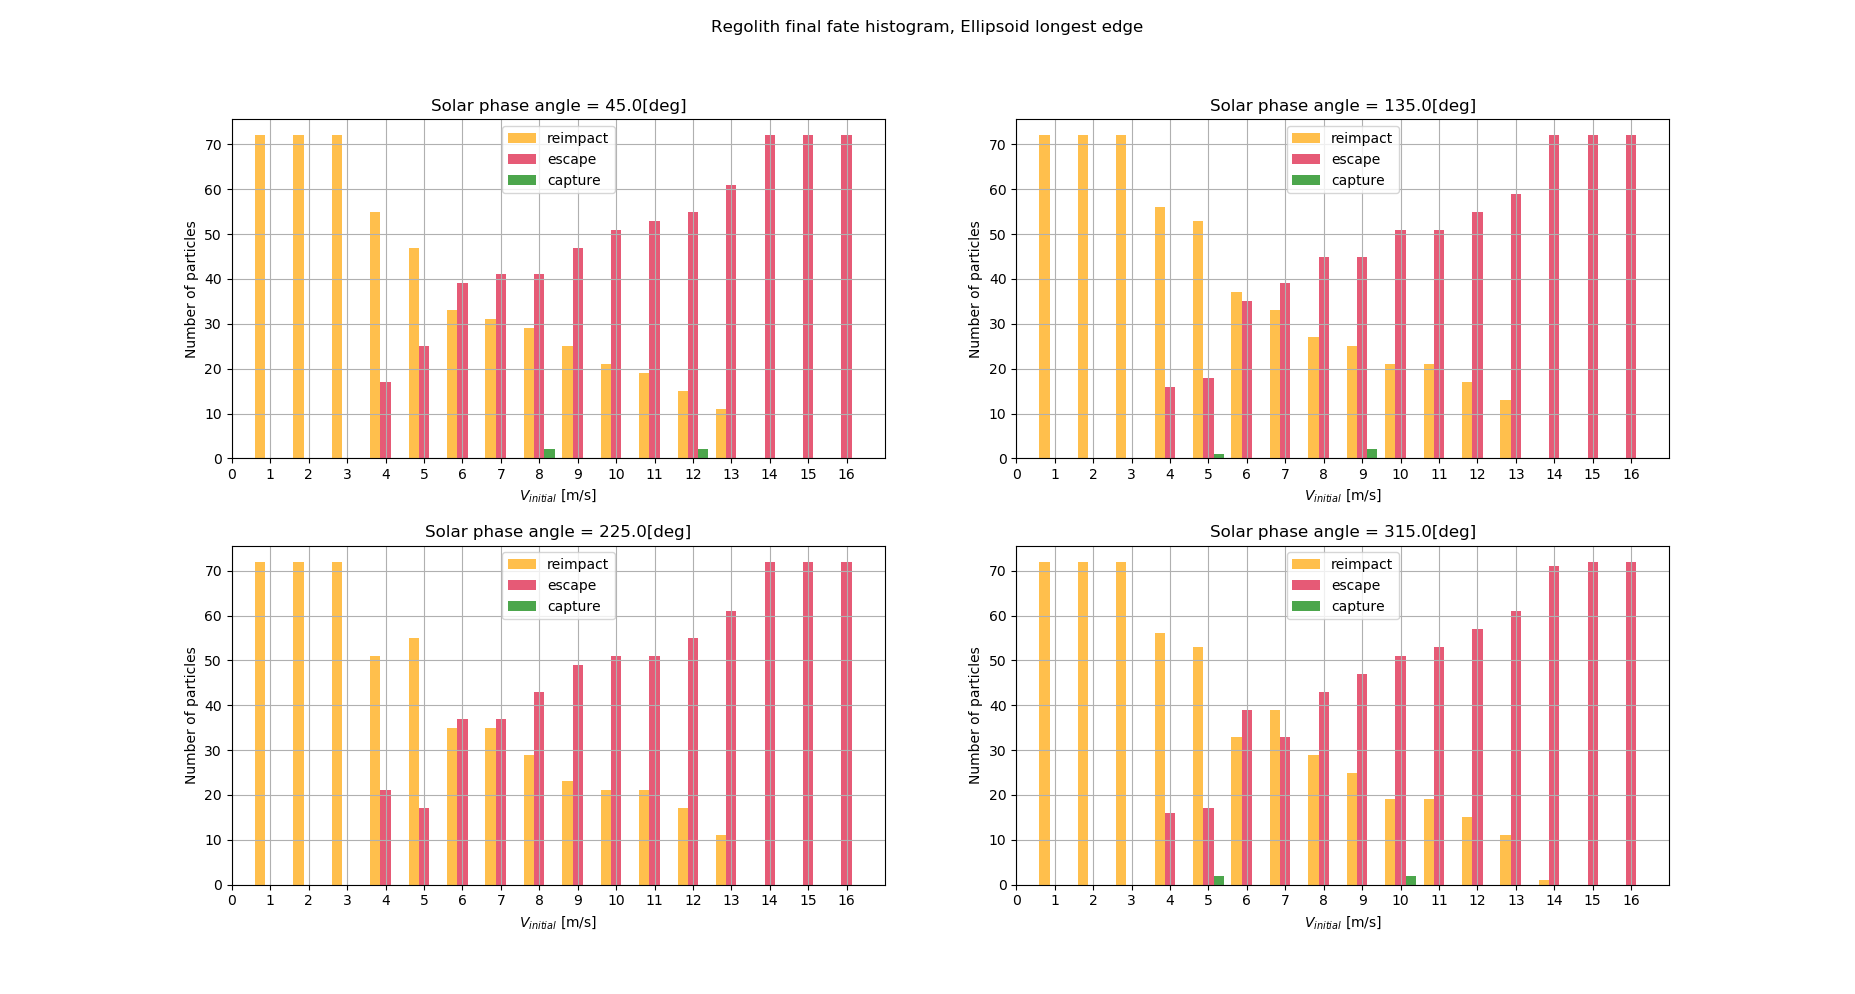
\includegraphics[angle=90, width=\textwidth, height=\textheight]{longest_edge_perturbations/3.2Density_1cmSize/final_fate_versus_launch_velocity_histogram_all_solar_phases.png}
\caption{Histogram showing the number of particles that re-impact, escape, or get captured around the asteroid, for different initial launch velocities. Particle code LoGSP-1.}
\label{fig:LoGSP_1_final_fate_histogram}
\end{figure}
\FloatBarrier
%%%
\Cref{fig:LoGSP_1_crashmap} depicts the surface distribution of regolith that re-impacts the surface when launched from the same location with different velocities and different initial Solar phase angles. The launch location is in the centre of the map, Latitude 0.0 [deg] and Longitude 0.0 [deg]. The particle distribution is the same for regions close to the launch point and for lower launch velocities up until 8.0 [m/s]. A similarity in distribution pattern is also observed around Longitude -150.0 [deg] for launch velocity of 9.0 [m/s] and around Longitude 150.0 [deg] for launch velocity of 10.0 [m/s] for the four Solar phase angles. The distribution pattern, for all launch velocities and initial Solar phases, is also symmetric about the equator. Again, the reason for this is the same as mentioned earlier for the symmetry in capture cases in \Cref{tab:LoGSP_1_capture}. Keeping the launch direction and velocity constant, we see that the distribution of regolith that re-impacts the surface does not change drastically with varying initial Solar phase angles, except for a relatively few cases. This is much easily observed in a plot of Range from the launch direction to the re-impact point versus launch azimuth for different velocities as shown in \Cref{fig:LoGSP_1_range_comparison}.

We haven't shown the range to re-impact point plots in \Cref{fig:LoGSP_1_range_comparison} for all launch velocities because the intention here is to show the qualitative behavior, which can be achieved by considering only a subset of the launch velocities that result in a re-impact scenario. The very first thing we observe is that as the launch velocity increases, the range of launch azimuth over which the regolith re-impacts the surface reduces because a higher velocity allows the regolith to enter a higher orbit (as it attains a relatively higher energy) and reduces the probability of a re-impact. Even as the velocity increases, we see that the azimuths that result in a re-impact are the ones in which the regolith is launched in a direction that is opposite to the asteroid's rotation direction. This makes sense since the regolith's energy would be reduced the most in this scenario compared to all other launch directions, thereby increasing the chances of a re-impact.

Now the primary purpose of the plots in \Cref{fig:LoGSP_1_range_comparison} (combined with \Cref{fig:LoGSP_1_crashmap}) is to depict the qualitative effect of Solar perturbations, for varying initial Solar phase angles, on the re-impact behavior of regolith compared to the case when no Solar perturbations are considered. For launch velocities of 4.0, 7.0 and 10.0 [m/s], we see that the Solar perturbations do not affect the re-impact location for cases when the particle is launched in directions opposite to that of the asteroid's rotation. However, we do see few exceptions to the former statement, most noticeably in the case of 7.0 [m/s]. But for the majority of cases where the re-impact location remains unchanged, we see from \Cref{fig:LoGSP_1_reimpact_time}, that these particles spend less than 3.0 [Hrs] in orbit which is not enough time for the Solar perturbations to act and have any significant impact on the dynamics of the particles. So in essence this is what's happening here - Particles when launched in a direction that is opposite to that of the asteroid's rotation, even at relatively high velocities such as 10.0 [m/s], loose enough energy to stay in a relatively lower orbit (see \Cref{fig:LoGSP_1_maxAltitude_reimpactscenario}) where the gravitational force of the asteroid is significantly stronger than any of the Solar perturbations and as the particle spends a very short time in orbit before re-impact, the Solar perturbations do not get enough time to affect the particle's orbit and hence the particle re-impacts the same location as it would have when no Solar perturbations were considered in the simulation. For the lower launch velocities of 4.0 and 7.0 [m/s], the differences in re-impact locations are more pronounced when the regolith is launched in the same direction as that of the asteroid's rotation. Particles gain relatively higher energy in this case, enter a higher orbit and spend enough time in there for the Solar perturbations to affect it's motion. For the case of the launch velocity of 13.0 [m/s] in \Cref{fig:LoGSP_1_range_comparison}, the velocity is high enough such that the particle does not loose enough energy when launched opposite to the asteroid's rotational direction and is able to enter a relatively higher orbit (see \Cref{fig:LoGSP_1_maxAltitude_reimpactscenario}) and stay there for a relatively longer time, as seen in \Cref{fig:LoGSP_1_reimpact_time}, which results in the Solar perturbations affecting the orbital motion and eventually the re-impact location of the regolith.
%%%
\begin{figure}[htb]
\centering
\captionsetup{justification=centering}
% another option for includegraphics - keepaspectratio
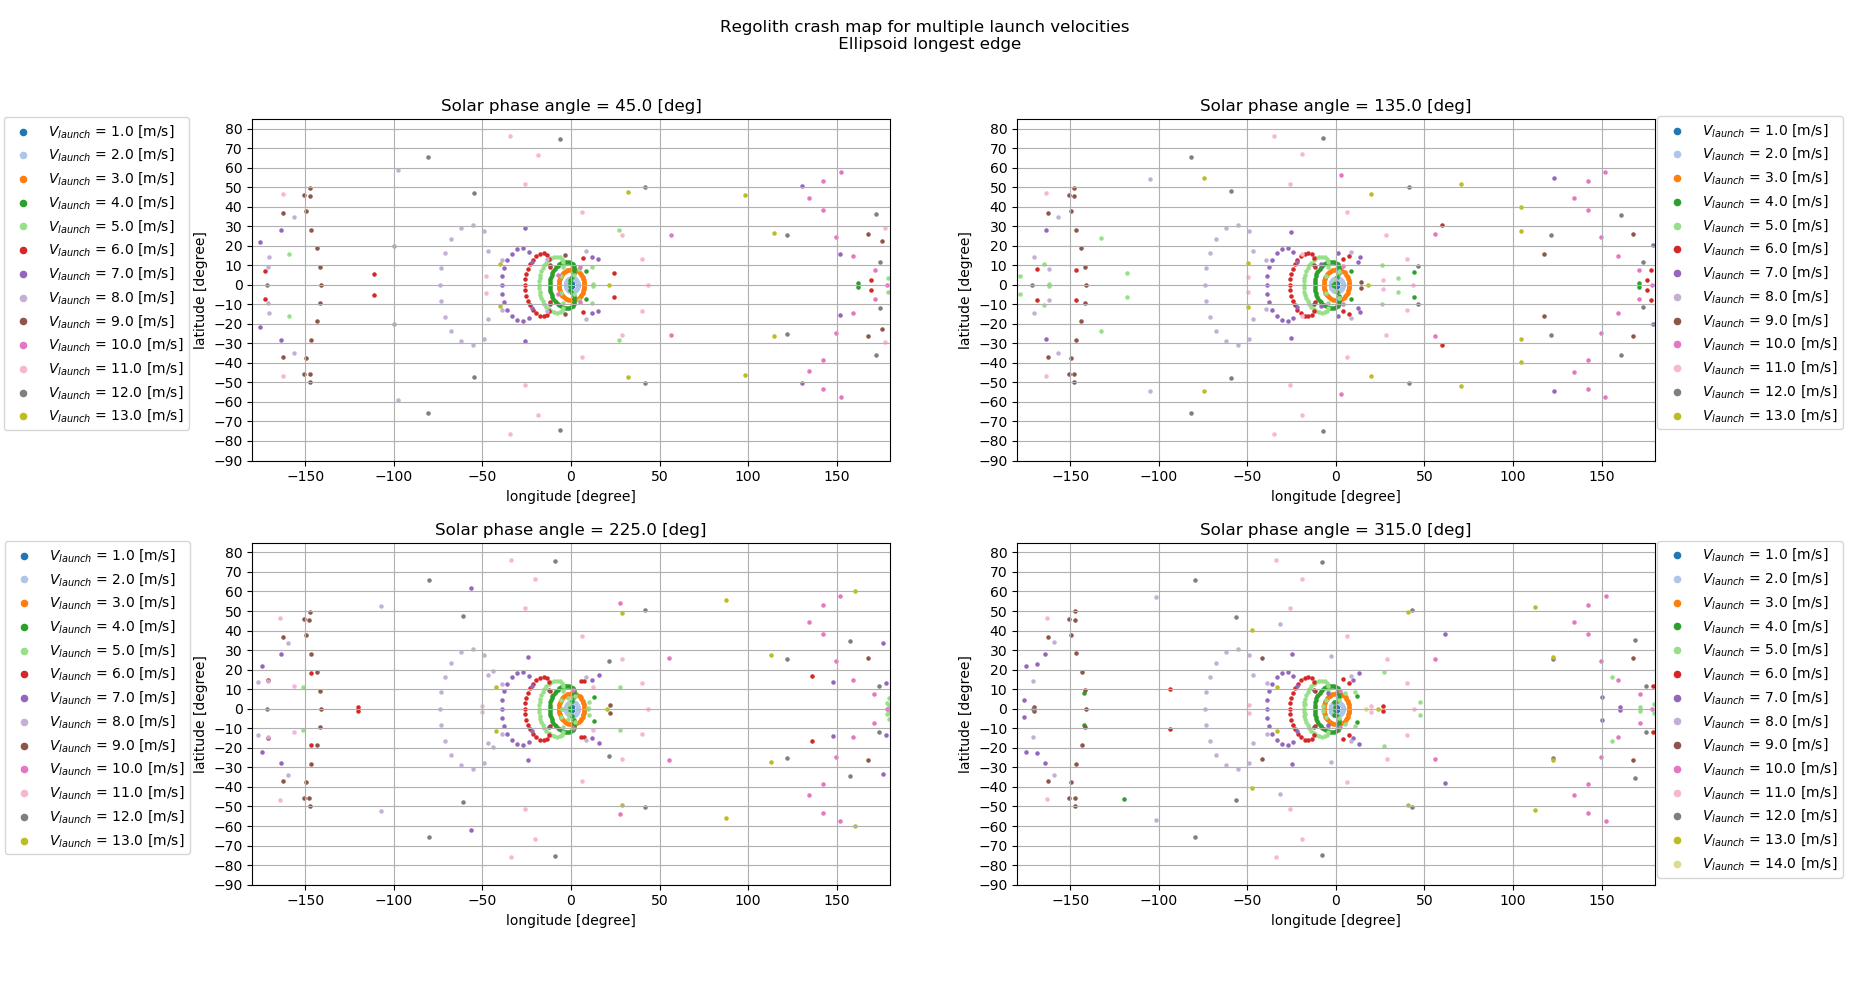
\includegraphics[angle=90, width=\textwidth, height=\textheight]{longest_edge_perturbations/3.2Density_1cmSize/crash_map_all_solar_phases.png}
\caption{Surface distribution of re-impacted regolith for different launch velocities. The launch location is \\ latitude: 0.0 [deg], longitude: 0.0 [deg]. Particle code LoGSP-1.}
\label{fig:LoGSP_1_crashmap}
\end{figure}
\FloatBarrier
%%%
%%%
\begin{figure}[htb]
\centering
\captionsetup{justification=centering}
% another option for includegraphics - keepaspectratio
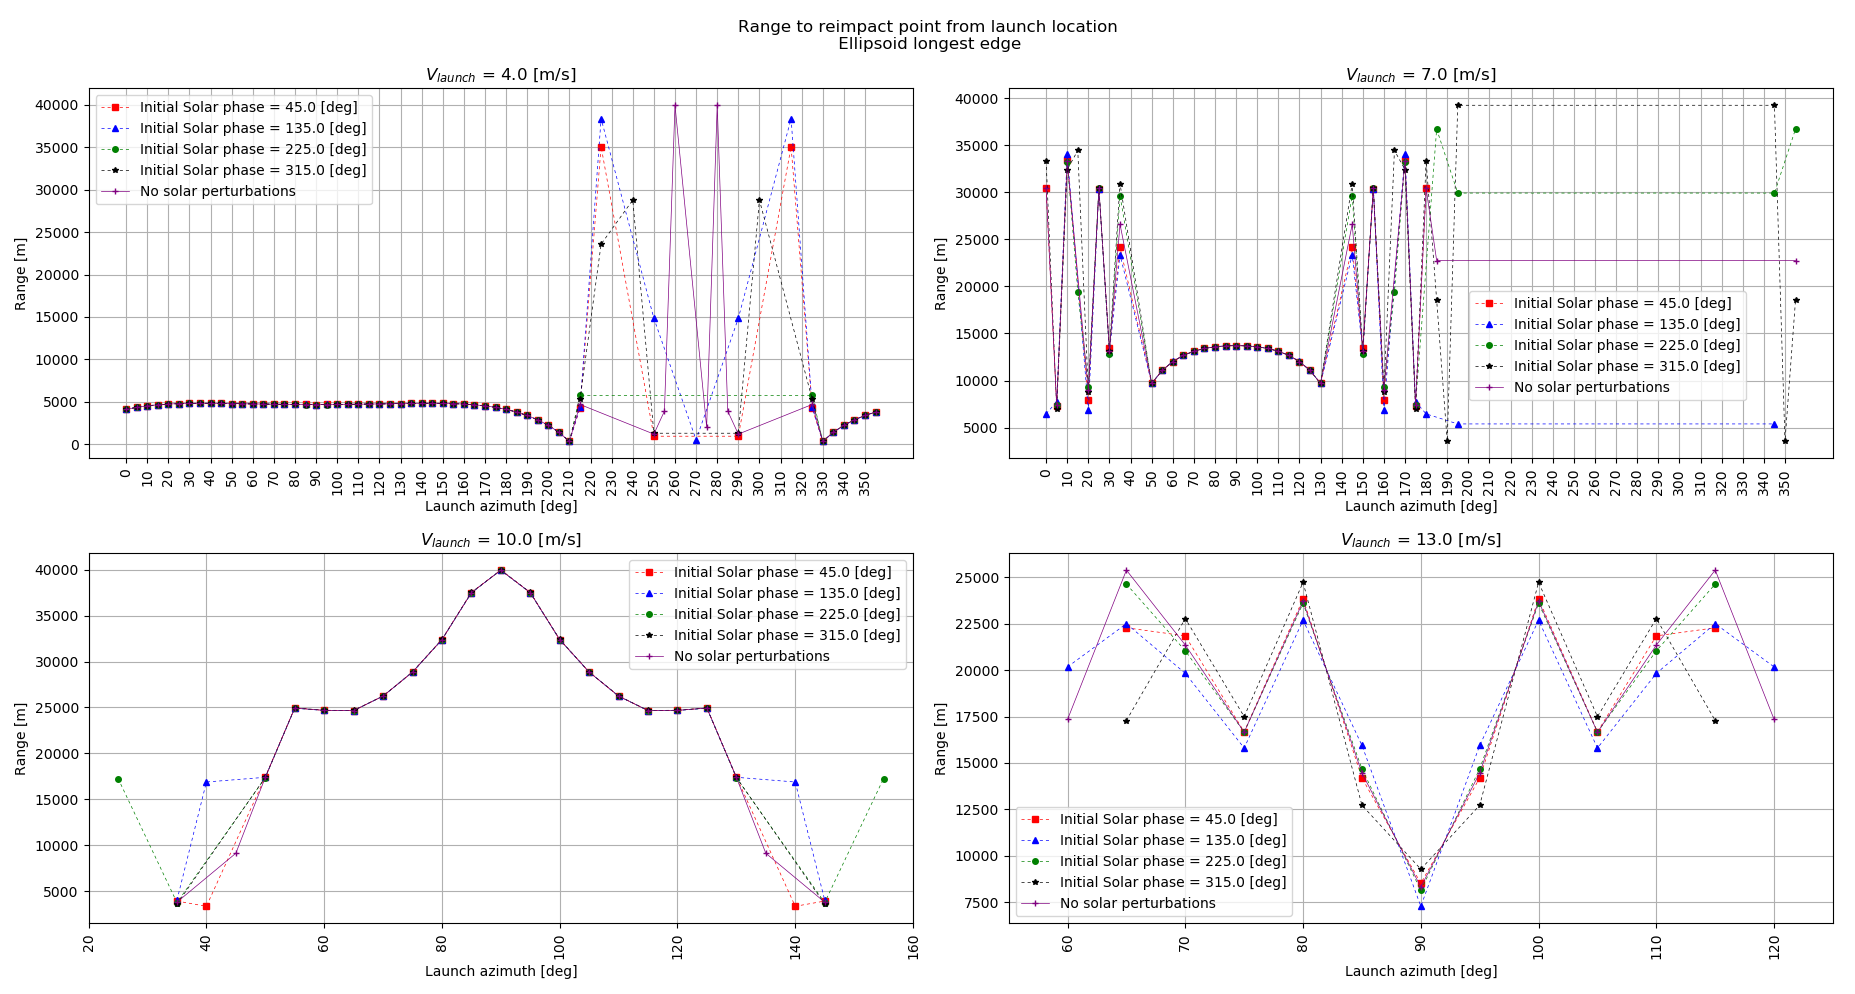
\includegraphics[angle=90, width=\textwidth, height=\textheight]{longest_edge_perturbations/3.2Density_1cmSize/reimpactRangeComparison.png}
\caption{Range to re-impact location from the launch point for different velocities. Particle code LoGSP-1.}
\label{fig:LoGSP_1_range_comparison}
\end{figure}
\FloatBarrier
%%%
%%%
\begin{figure}[htb]
\centering
\captionsetup{justification=centering}
% another option for includegraphics - keepaspectratio
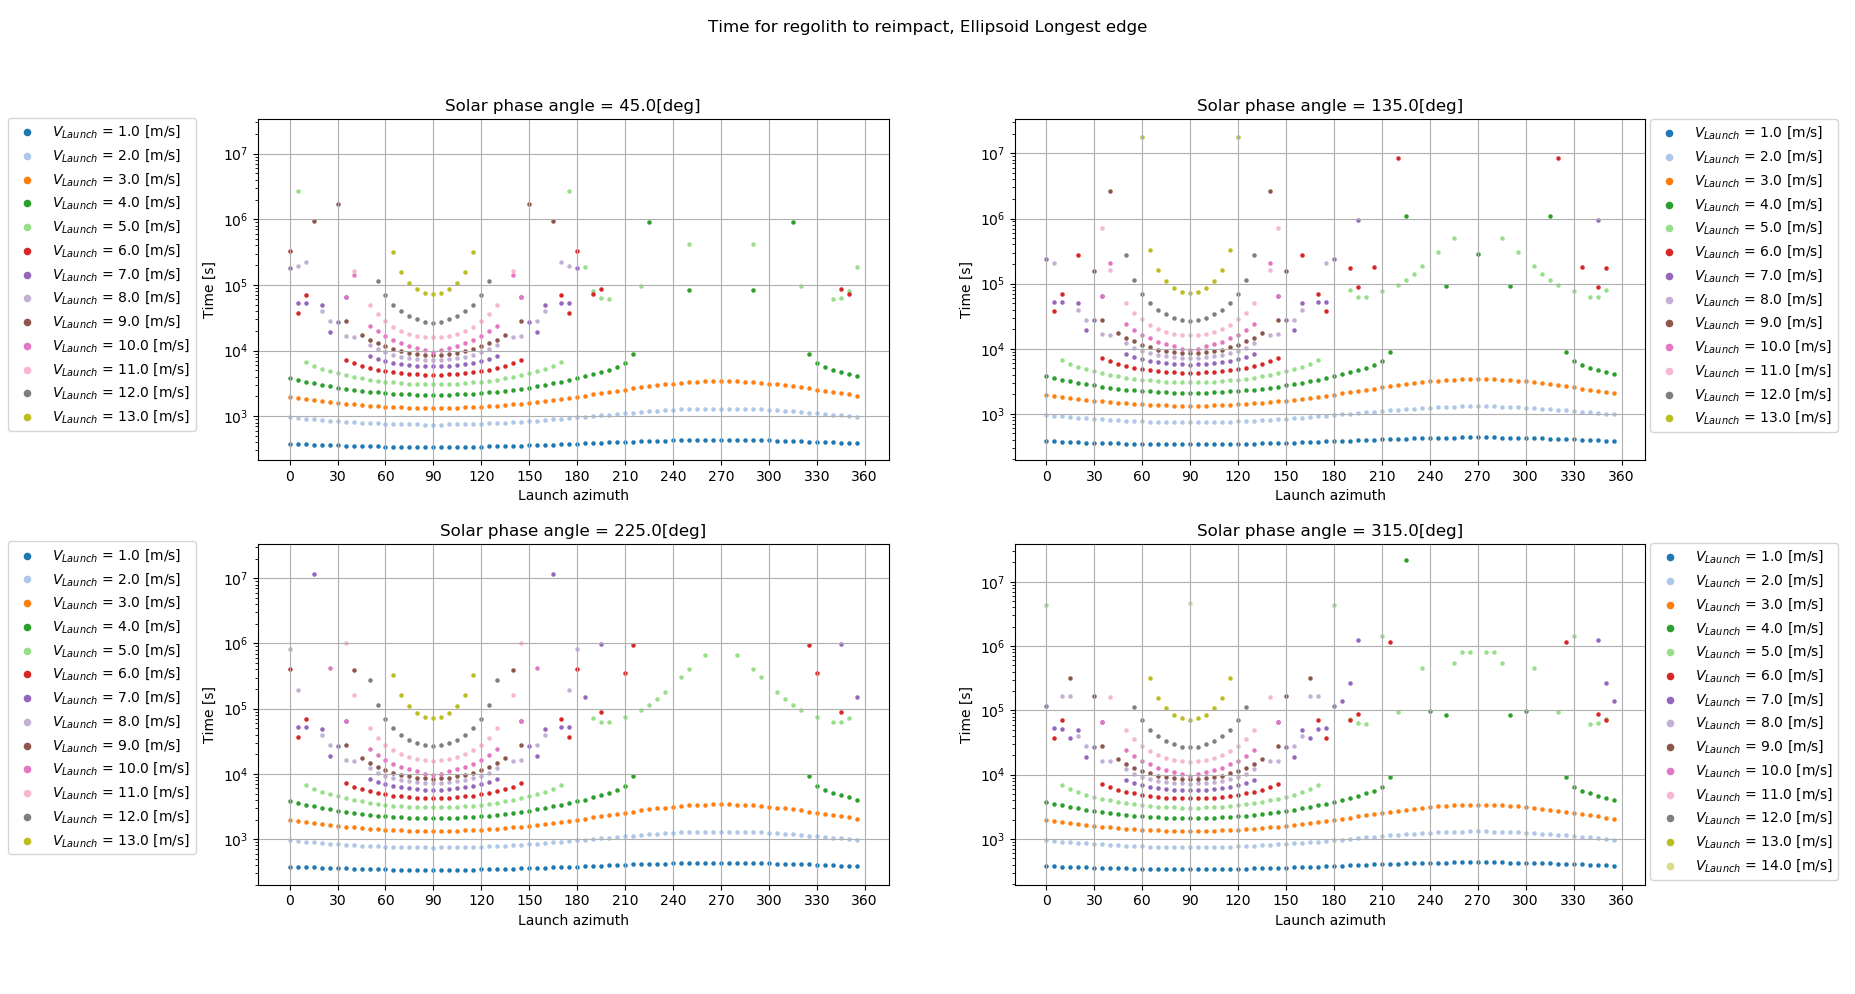
\includegraphics[angle=90, width=\textwidth, height=\textheight]{longest_edge_perturbations/3.2Density_1cmSize/time_to_reimpact_all_solar_phases.png}
\caption{Time taken by regolith at different velocities and launch directions to re-impact with the surface of the asteroid. Particle code LoGSP-1.}
\label{fig:LoGSP_1_reimpact_time}
\end{figure}
\FloatBarrier
%%%
We shall now look at the cases where the lofted regolith gets (temporarily) captured in orbit by the asteroid. The initial conditions for all capture cases, for the current particle size and density, were mentioned earlier in \Cref{tab:LoGSP_1_capture}. \Cref{fig:LoGSP_1_capture_orbital_range} depicts the progression in orbital range of the temporarily captured regolith. The straight lines in the plot are used to mark the different altitude regimes. These are the \gls{LAO}, \gls{MAO}, \gls{HAO}, \gls{UHAO}, and \gls{EHAO}. These altitude regime definitions are not from well defined standards, but instead were arbitrarily chosen as integer multiples of the longest semi-major axis, $\alpha$, of the tri-axial ellipsoid shaped asteroid. The definition for these altitude regimes is given in \Cref{tab:altitude_regimes}.
%%%
\begin{table}[htb]
\centering
\captionsetup{justification=centering}
\caption{Altitude regimes and their definitions}
\label{tab:altitude_regimes}
\begin{tabular}{|c|c|}
\hline
\textbf{Altitude regime}        & \textbf{Definition}                    \\ \hline
\gls{LAO}                       & Asteroid surface to $2 \times \alpha$  \\ \hline
\gls{MAO}                       & $2 \times \alpha$ to $3 \times \alpha$ \\ \hline
\gls{HAO}                       & $3 \times \alpha$ to $5 \times \alpha$ \\ \hline
\gls{UHAO}                      & $5 \times \alpha$ to $7 \times \alpha$ \\ \hline
\gls{EHAO}                      & Above $7 \times \alpha$                \\ \hline
\end{tabular}
\end{table}
\FloatBarrier
%%%
The purpose of plotting data as shown in \Cref{fig:LoGSP_1_capture_orbital_range} was to look for any patterns or periodicity, if they existed, and to see if particles in temporary capture scenario remain closer to the asteroid or further away from it. The symmetry as explained for initial conditions mentioned in \Cref{tab:LoGSP_1_capture} can also be seen in \Cref{fig:LoGSP_1_capture_orbital_range}, for example, regolith launched with velocity of 8.0 [m/s] and launch azimuth of 15.0 [deg] (shown by the purple curve in the top plot in \Cref{fig:LoGSP_1_capture_orbital_range}) shows the same behavior as that of regolith launched with the same velocity and 165.0 [deg] launch azimuth (shown by the green curve in the bottom plot in \Cref{fig:LoGSP_1_capture_orbital_range}). Another thing we see from the plot is that, apart from case number 11 in \Cref{tab:LoGSP_1_capture}, the captured regolith stay in the higher altitude regions for most part and only briefly do they fall within the \gls{MAO} and \gls{LAO} region. We shall now look at atleast three cases from \Cref{fig:LoGSP_1_capture_orbital_range} in a bit more detail to understand the effect of Solar perturbations by comparing these cases with their counterparts from the simulation where Solar perturbations were omitted.

Of all the cases shown in \Cref{fig:LoGSP_1_capture_orbital_range} or \Cref{tab:LoGSP_1_capture}, the one with a launch velocity of 10.0 [m/s] and launch azimuth of 45.0 [deg] results in a re-impact scenario when Solar perturbations are omitted but the same initial conditions lead to a temporary capture orbit when perturbations were added for an initial Solar phase angle of 315.0 [deg]. Every other initial condition for the capture cases had otherwise resulted in an escape situation when simulations were conducted without the Solar perturbations. The 3D trajectory plot in two different views for the former case are shown in \Cref{fig:LoGSP_1_capture_case_5_3d_traj_inertialFrame_differnetViews} (see \Cref{fig:LoGSP_1_capture_case_5_3d_trajectory} also for the 3D trajectory representation in body fixed frame). The 2D trajectory for the same is shown in \Cref{fig:LoGSP_1_capture_case_5_2d_traj_inertialFrame} in inertial frame and in \Cref{fig:LoGSP_1_capture_case_5_2d_traj_bodyFrame} in the asteroid centric rotating frame or the body frame. The web-link or URL for the trajectory animation of the particle (in inertial frame and in XY plane only) can be found in \Cref{fig:LoGSP_1_capture_case_5_2d_trajectory_animation}.
%%%
\begin{figure}[htb]
\centering
\captionsetup{justification=centering}
% another option for includegraphics - keepaspectratio

\includegraphics[scale=0.25]{longest_edge_perturbations/3.2Density_1cmSize/qrcode_10ms_45Azimuth_315SolarPhase.png}
\caption{2D trajectory animation (XY Plane) of capture regolith for case number 5 in \Cref{tab:LoGSP_1_capture}. Particle code LoGSP-1. Scan the QR code to view the animation or use the following web-link: \url{https://youtu.be/oZDhDo5CIsk}}
\label{fig:LoGSP_1_capture_case_5_2d_trajectory_animation}
\end{figure}
\FloatBarrier
%%%
%%%
\begin{figure}[p]
\centering
\captionsetup{justification=centering}
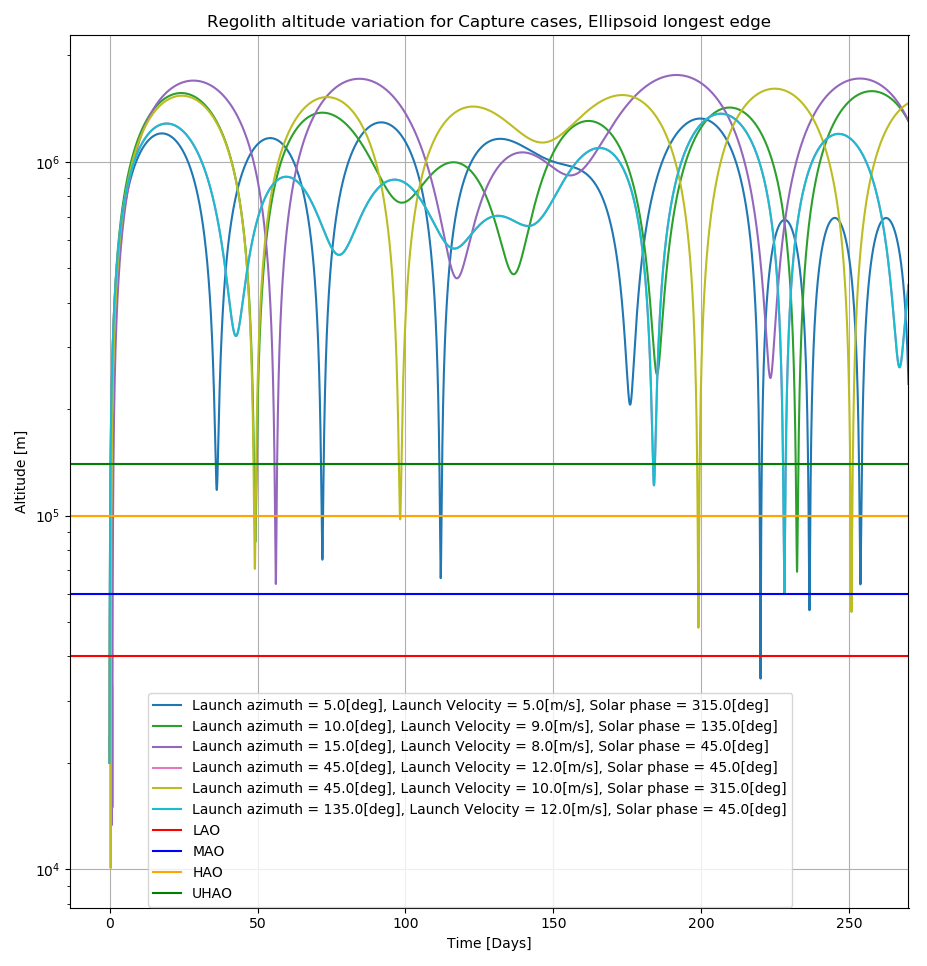
\includegraphics[scale=0.5]{longest_edge_perturbations/3.2Density_1cmSize/altitude_versus_time_all_cases_part_1.png}
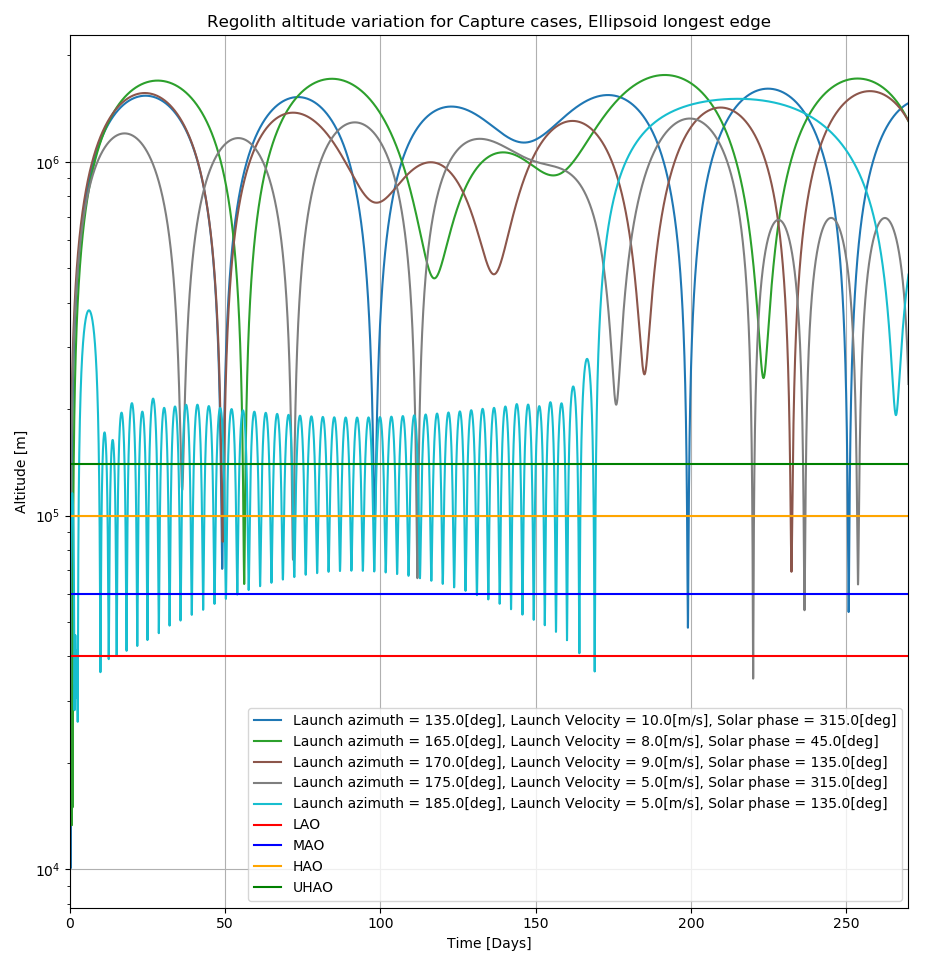
\includegraphics[scale=0.5]{longest_edge_perturbations/3.2Density_1cmSize/altitude_versus_time_all_cases_part_2.png}
\caption{Orbital range progression with time for temporary capture scenarios. Particle code LoGSP-1.}
\label{fig:LoGSP_1_capture_orbital_range}
\end{figure}
\FloatBarrier
%%%
%%%
\begin{figure}[htb]
\centering
\captionsetup{justification=centering}
% another option for includegraphics - keepaspectratio
\subfloat[]{
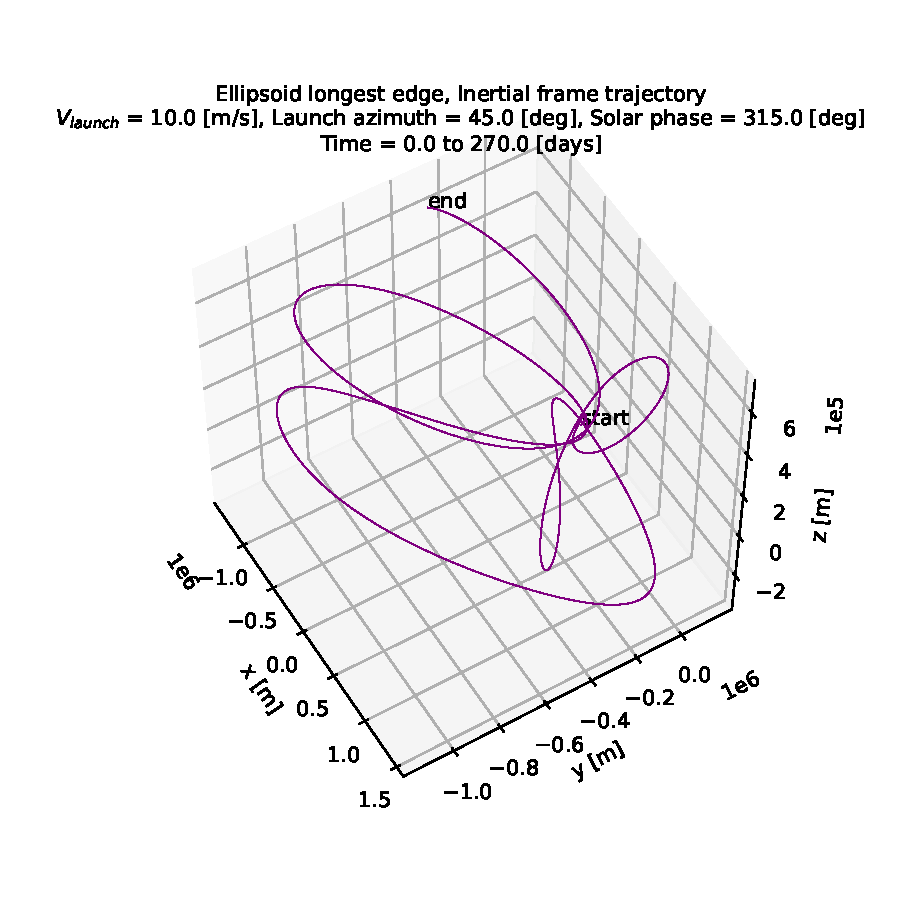
\includegraphics[width=\textwidth, height=0.5\textheight, keepaspectratio=true]{longest_edge_perturbations/3.2Density_1cmSize/3dTrajectory_10ms_45Azimuth_315solarPhase_inertialFrame_View1.pdf}
}

\subfloat[]{
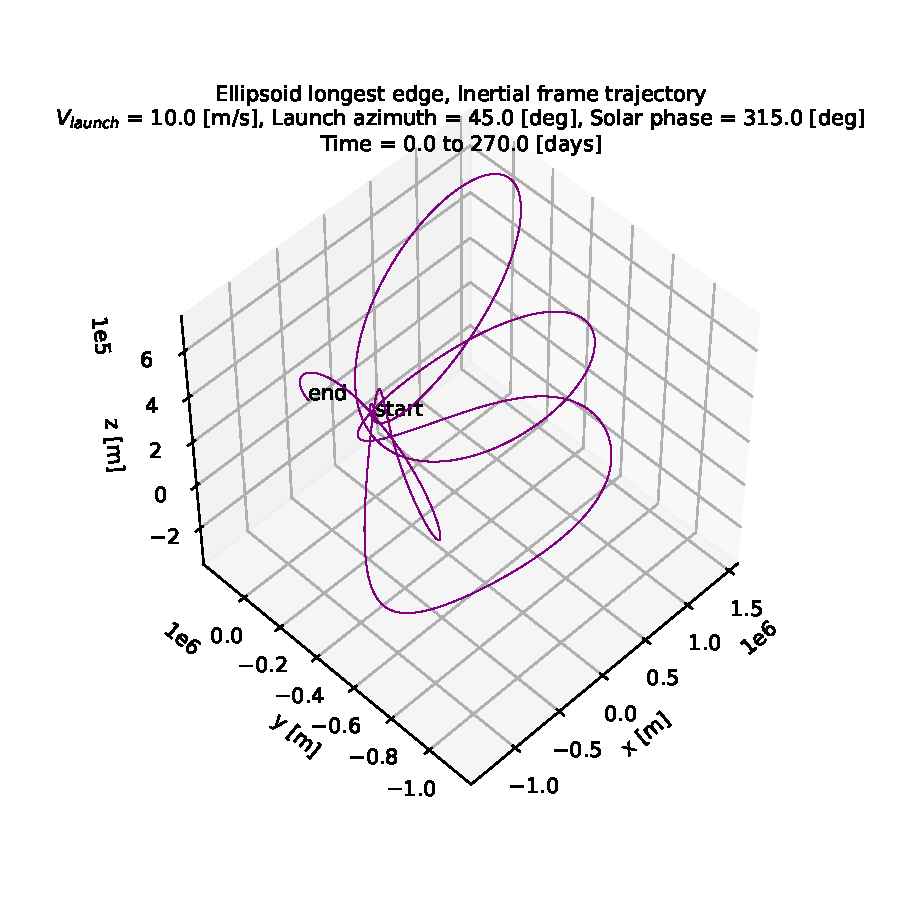
\includegraphics[width=\textwidth, height=0.5\textheight, keepaspectratio=true]{longest_edge_perturbations/3.2Density_1cmSize/3dTrajectory_10ms_45Azimuth_315solarPhase_inertialFrame_View2.pdf}
}
\caption{3D inertial frame trajectory of capture regolith for case number 5 in \Cref{tab:LoGSP_1_capture} in two different viewing angles. Particle code LoGSP-1.}
\label{fig:LoGSP_1_capture_case_5_3d_traj_inertialFrame_differnetViews}
\end{figure}
\FloatBarrier
%%%
Note that in the trajectory animation in \Cref{fig:LoGSP_1_capture_case_5_2d_trajectory_animation} (and any other animation included henceforth) the particle is made to skip several data points in between along the trajectory when it is far away from the asteroid, just to reduce the length of the animation. So because of this, the particle appears to be moving faster when it is away from the asteroid but this is not true. For the exact velocity of the particle, the reader should look at the velocity magnitude indicator within the animation itself.

The animation shows that the particle reverses its direction of motion twice in its entire course. To visualize how this is happening in 3D, look at \Cref{fig:LoGSP_1_capture_case_5_3d_traj_inertialFrame_differnetViews}. The reason for this can be understood by looking at the direction of the perturbing acceleration, the gravitational acceleration vectors, and the combined effect of all accelerations acting on the particle. The direction of \gls{SRP} and \gls{STBE} are shown in \Cref{fig:LoGSP_1_capture_case_5_2d_trajectory_srp_stbe_perturbationVectors} and that of the net effect of the two is shown in \Cref{fig:LoGSP_1_capture_case_5_2d_trajectory_totalPerturbationVectors}. In the trajectory simulator, the gravity model (triaxial ellipsoid model) computes the acceleration in the rotating frame. We calculated the direction of the gravitational acceleration in inertial frame in post-simulation analysis assuming a point-mass model by considering the fact that when the regolith is far-away from the asteroid, its gravity field would appear as that of a point-mass gravity source. The gravitational acceleration vectors are shown in \Cref{fig:LoGSP_1_capture_case_5_2d_trajectory_gravityVector}. The net acceleration acting on the particle is then shown in \Cref{fig:LoGSP_1_capture_case_5_2d_totalAccelerationVector_inertialFrame}. All acceleration vectors are shown along those parts of the trajectory where the magnitude of \gls{SRP} acceleration is of the same order of magnitude as that of the gravitational acceleration. However, the magnitude of the \gls{STBE} acceleration is always 1.0 order of magnitude smaller than the gravitational acceleration for those very same points along the trajectory, but is still significant. We do not show the vectors for the entire trajectory for two reasons; first, when close to the asteroid the direction of these vectors would reduce the clarity of the plot and,  second, we want to discuss the effect of the perturbations when the particle is far away from the asteroid because then they are as significant as the gravitational force.

In \Cref{fig:LoGSP_1_capture_case_5_2d_traj_inertialFrame}, the trajectory loops numbered 1 and 2 (XY plane), is where the particle's direction of motion gets reversed. If we look at \Cref{fig:LoGSP_1_capture_case_5_2d_trajectory_srpVectors}, we see that the direction of the \gls{SRP} vector is consistent with how the particle changes its direction of motion. This, however, does not mean that the \gls{SRP} is the sole actor responsible for how the particle's motion eventually turns out to be (and we will see this in detail shortly). The direction of \gls{STBE}, as shown in \Cref{fig:LoGSP_1_capture_case_5_2d_trajectory_stbeVectors}, however, does not directly tell us on how the particle's motion would change as it progresses through its trajectory. \gls{STBE} is always an order of magnitude smaller than \gls{SRP} for the points shown in the two plots and its direction is not consistent with how the particle changes its direction of motion but its contribution to the capture scenario is significant (we will see the effect of removing \gls{STBE} shortly). The direction of the net perturbing acceleration, shown in \Cref{fig:LoGSP_1_capture_case_5_2d_trajectory_totalPerturbationVectors}, shows us exactly how and where the motion of the particle is directed. Especially when we look at trajectory loops 1 and 2 in \Cref{fig:LoGSP_1_capture_case_5_2d_traj_inertialFrame}, we can see that the net perturbing vector is acting in the direction that is consistent with how the particle changes its orbital motion. Now looking at these plots that we just discussed, a question that arises is that - why did the particle remain in a temporary capture orbit, and for example not escape especially when the net perturbing acceleration was acting opposite to the direction of asteroid such as in trajectory loop number 3 in \Cref{fig:LoGSP_1_capture_case_5_2d_traj_inertialFrame}? The answer to this is found by looking at the direction of gravitational attraction in \Cref{fig:LoGSP_1_capture_case_5_2d_trajectory_gravityVector} and the total acceleration (i.e. the net effect of gravity and perturbations) acting on the particle in \Cref{fig:LoGSP_1_capture_case_5_2d_totalAccelerationVector_inertialFrame}. Although the gravitational acceleration has the same order of magnitude as that of the Solar perturbations when the particle is far away from the asteroid, we see that the net effect of the two is towards the asteroid and hence prevents the particle from escaping.
%%%
\begin{figure}[htb]
\centering
\captionsetup{justification=centering}
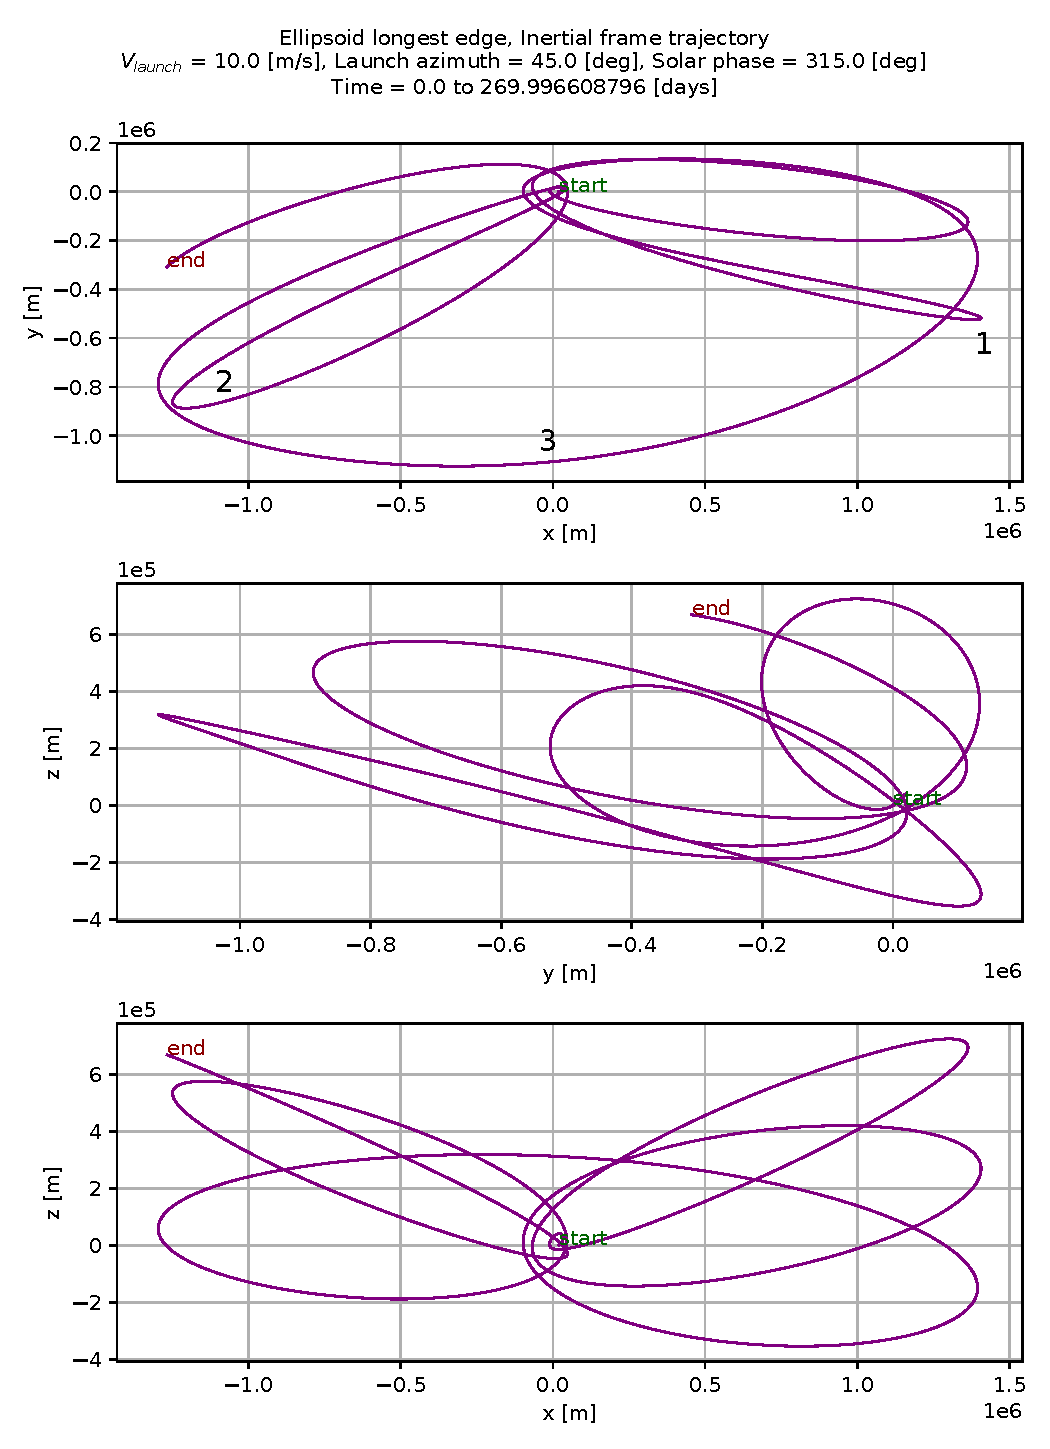
\includegraphics[width=\linewidth, height=\textheight, keepaspectratio=true]{longest_edge_perturbations/3.2Density_1cmSize/10ms_45Azimuth_315SolarPhase/2d_trajectory_inertialFrame_edit.pdf}
\caption{2D inertial frame trajectory of capture regolith for case number 5 in \Cref{tab:LoGSP_1_capture}. Particle code LoGSP-1.}
\label{fig:LoGSP_1_capture_case_5_2d_traj_inertialFrame}
\end{figure}
\FloatBarrier
%%%
%%%
\begin{figure}[htb]
\centering
\captionsetup{justification=centering}
\subfloat[]
{
    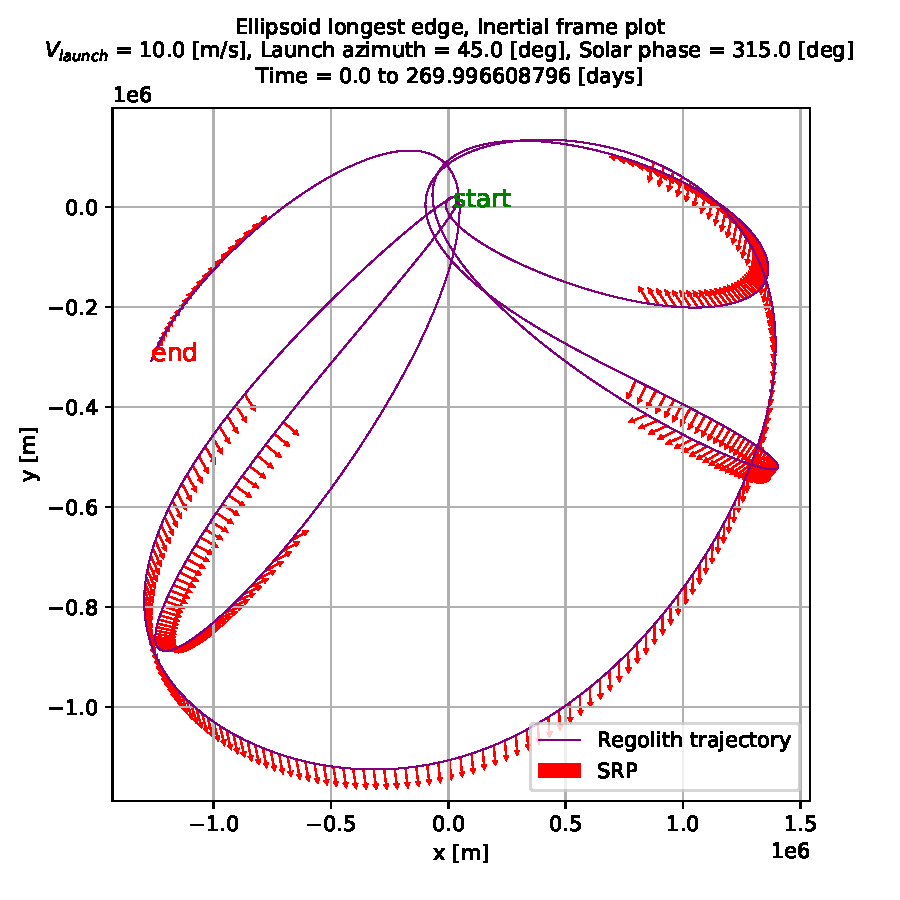
\includegraphics[width=\linewidth, height=0.45\textheight, keepaspectratio=true]{longest_edge_perturbations/3.2Density_1cmSize/10ms_45Azimuth_315SolarPhase/srp_inertialFrame.pdf}
    \label{fig:LoGSP_1_capture_case_5_2d_trajectory_srpVectors}
}

\subfloat[]
{
    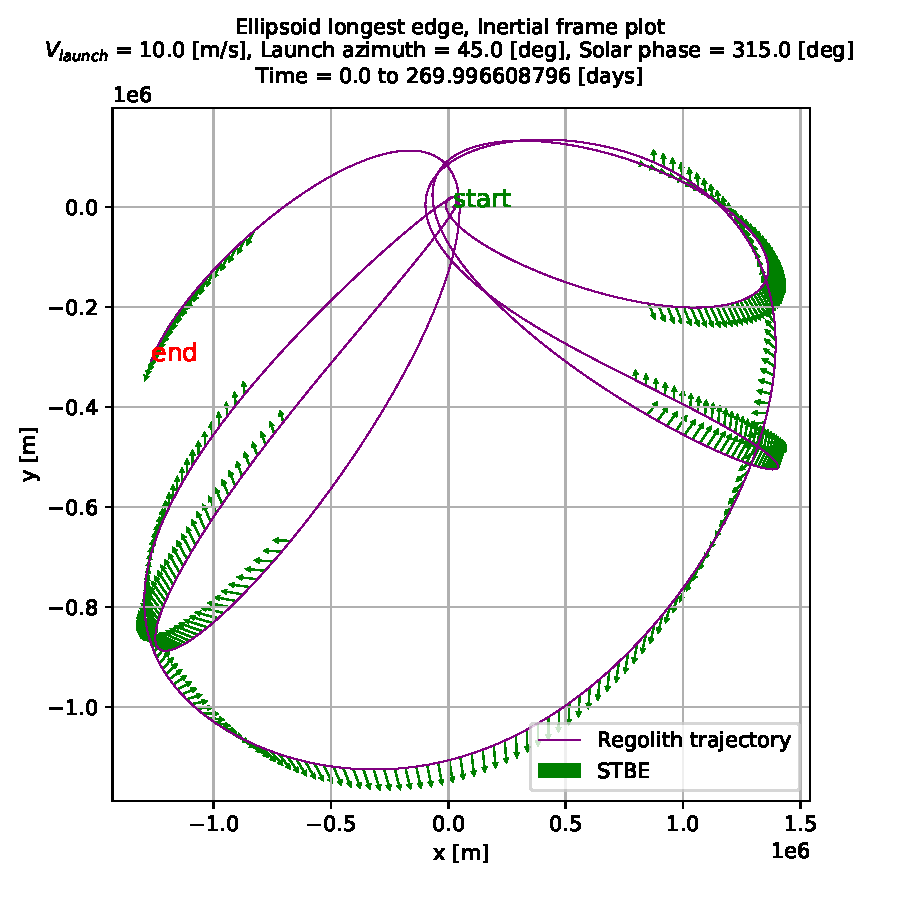
\includegraphics[width=\linewidth, height=0.45\textheight, keepaspectratio=true]{longest_edge_perturbations/3.2Density_1cmSize/10ms_45Azimuth_315SolarPhase/stbe_inertialFrame.pdf}
    \label{fig:LoGSP_1_capture_case_5_2d_trajectory_stbeVectors}
}
\caption{2D trajectory of capture regolith for case number 5 in \Cref{tab:LoGSP_1_capture} with direction of \gls{SRP} and \gls{STBE} perturbation vectors. Note that the vectors are shown only for those parts of the trajectory where the \gls{SRP} magnitude is of the same order as that of the asteroid's gravitational acceleration. For those very same points along the trajectory, the magnitude of the \gls{STBE} is always 1.0 order of magnitude smaller than the gravitational acceleration. Particle code LoGSP-1.}
\label{fig:LoGSP_1_capture_case_5_2d_trajectory_srp_stbe_perturbationVectors}
\end{figure}
\FloatBarrier
%%%
%%%
\begin{figure}[htb]
\centering
\captionsetup{justification=centering}
\subfloat[]{
    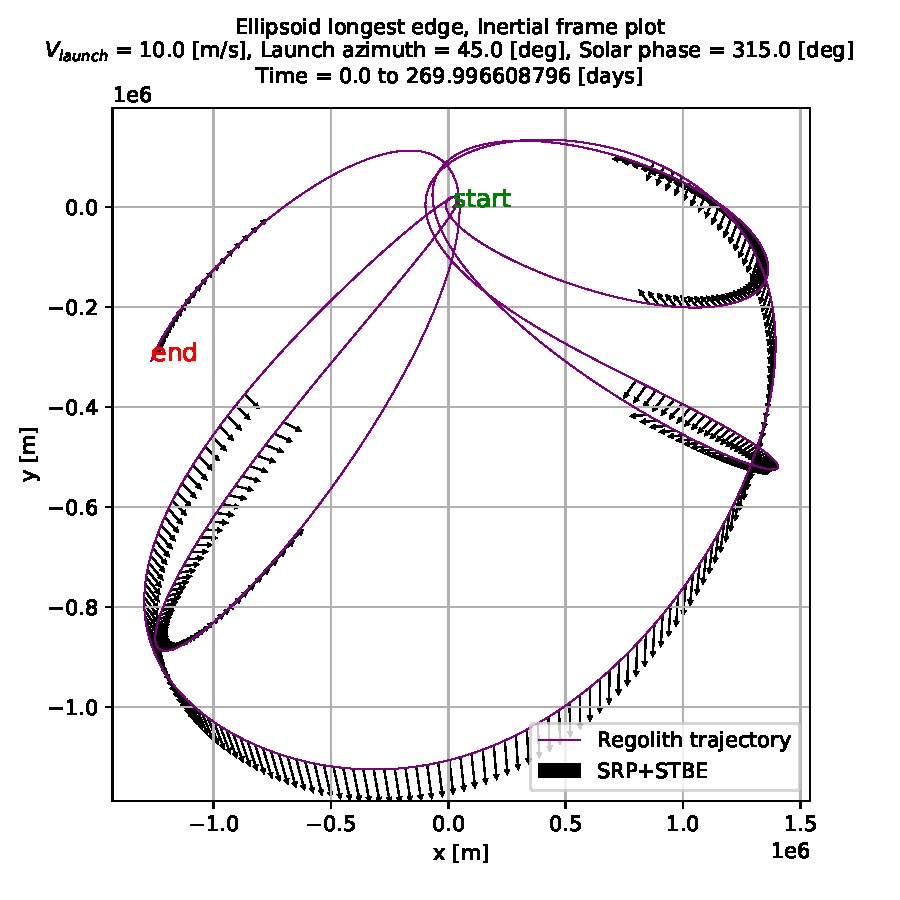
\includegraphics[width=\linewidth, height=0.45\textheight, keepaspectratio=true]{longest_edge_perturbations/3.2Density_1cmSize/10ms_45Azimuth_315SolarPhase/totalPerturbation_inertialFrame.pdf}
    \label{fig:LoGSP_1_capture_case_5_2d_trajectory_totalPerturbationVectors}
}

\subfloat[]
{
    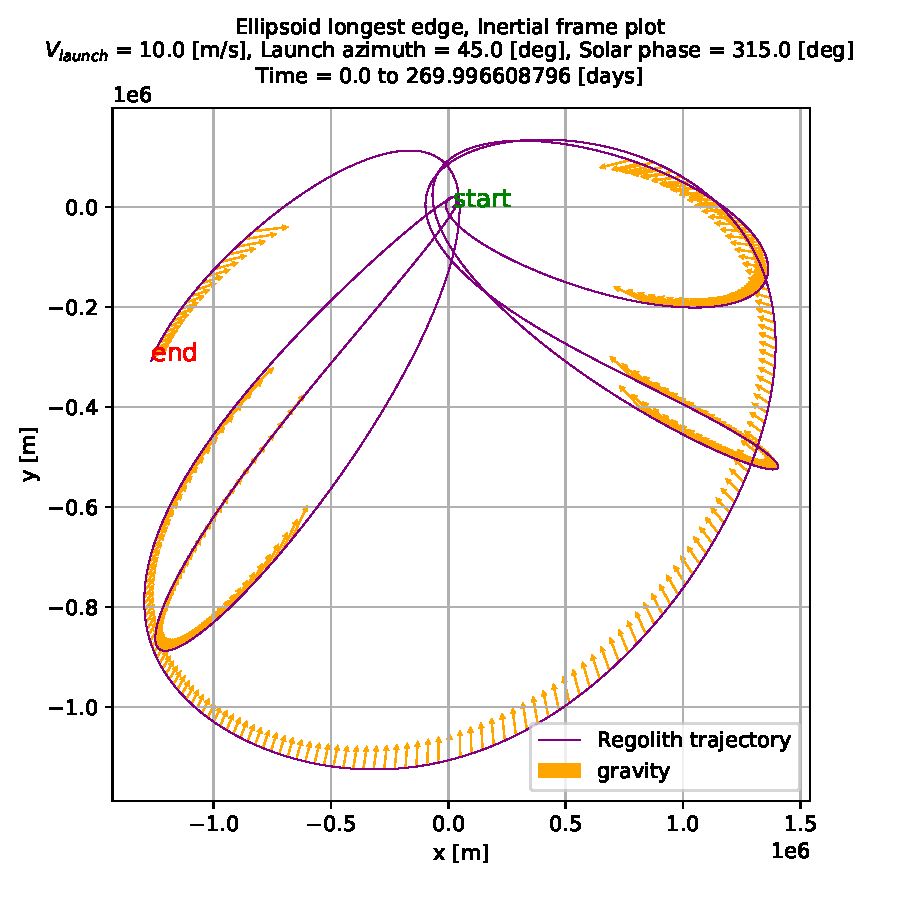
\includegraphics[width=\linewidth, height=0.45\textheight, keepaspectratio=true]{longest_edge_perturbations/3.2Density_1cmSize/10ms_45Azimuth_315SolarPhase/gravity_inertialFrame.pdf}
    \label{fig:LoGSP_1_capture_case_5_2d_trajectory_gravityVector}
}
\caption{2D trajectory of capture regolith for case number 5 in \Cref{tab:LoGSP_1_capture} with direction of the sum total of \gls{SRP} and \gls{STBE} perturbation vectors, and the direction of the gravitational acceleration vector for the same data points. Note that the vectors are shown only for those parts of the trajectory where the \gls{SRP} magnitude is of the same order as that of the asteroid's gravitational acceleration. For those very same points along the trajectory, the magnitude of the \gls{STBE} is always 1.0 order of magnitude smaller than the gravitational acceleration. Particle code LoGSP-1.}
\end{figure}
\FloatBarrier
%%%
%%%
\begin{figure}[htb]
\centering
\captionsetup{justification=centering}
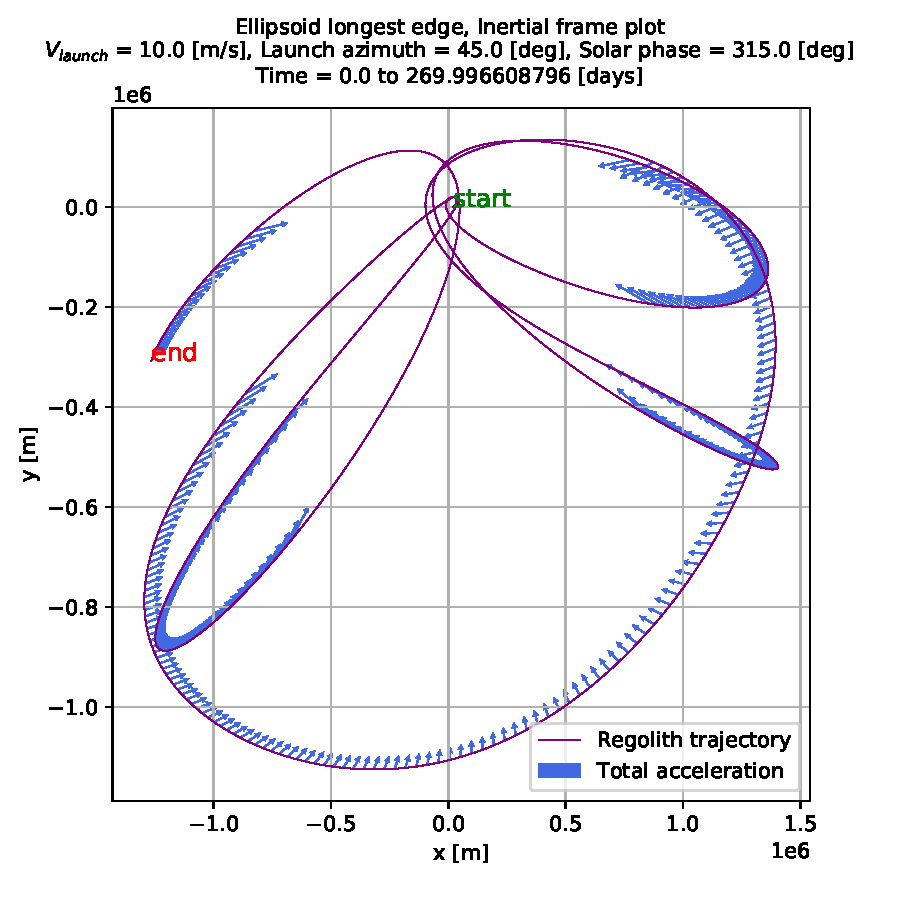
\includegraphics[width=\linewidth, height=0.45\textheight, keepaspectratio=true]{longest_edge_perturbations/3.2Density_1cmSize/10ms_45Azimuth_315SolarPhase/totalAcceleration.pdf}
\caption{2D trajectory of capture regolith for case number 5 in \Cref{tab:LoGSP_1_capture} with direction of the net acceleration vector. Note that the vectors are shown only for those parts of the trajectory where the \gls{SRP} magnitude is of the same order as that of the asteroid's gravitational acceleration. For those very same points along the trajectory, the magnitude of the \gls{STBE} is always 1.0 order of magnitude smaller than the gravitational acceleration. Particle code LoGSP-1.}
\label{fig:LoGSP_1_capture_case_5_2d_totalAccelerationVector_inertialFrame}
\end{figure}
\FloatBarrier
%%%
Both \gls{SRP} and \gls{STBE} together are necessary in getting the capture trajectory shown in \Cref{fig:LoGSP_1_capture_case_5_2d_traj_inertialFrame}. If either one of them is removed from the simulation, for the same launch conditions and initial Solar phase angle, then the results are completely different and we do not get a capture orbit. Note that the definition of capture orbit in this context implies that the particle stays in an orbit around the asteroid for the complete duration of 270.0 [days], i.e., the maximum time for which the simulation is run.

When only \gls{STBE} is removed, then we get a trajectory where the particle eventually escapes the asteroid. This is shown in \Cref{fig:LoGSP_1_capture_case_5_2d_inertialTrajectory_noSTBE}. The trajectory is completely different from the one in \Cref{fig:LoGSP_1_capture_case_5_2d_traj_inertialFrame}, even though the only difference between the two simulations is the omittion of \gls{STBE} perturbation. \Cref{fig:LoGSP_1_capture_case_5_2d_SRP_and_gravity_vector_noSTBE_inertialFrame} shows the direction of perturbing acceleration due to \gls{SRP} and the gravitational acceleration for those points along the trajectory where both have the same order of magnitude. The direction for the net acceleration acting on the particle is shown in \Cref{fig:LoGSP_1_capture_case_5_2d_totalAcceleration_vector_noSTBE_inertialFrame}. The trajectory of the particle starts out the same way in both \Cref{fig:LoGSP_1_capture_case_5_2d_inertialTrajectory_noSTBE} and \Cref{fig:LoGSP_1_capture_case_5_2d_traj_inertialFrame} however due to the lack of \gls{STBE} perturbation, the trajectories soon start to differ from each other. Upon comparing \Cref{fig:LoGSP_1_capture_case_5_2d_totalAccelerationVector_inertialFrame} and \Cref{fig:LoGSP_1_capture_case_5_2d_totalAcceleration_vector_noSTBE_inertialFrame} we can infer that the trajectories differ because the with the lack of \gls{STBE} the direction of the net acceleration vector differs for the two trajectories which eventually directs how the particle motion would progress. The particle trajectory in \Cref{fig:LoGSP_1_capture_case_5_2d_inertialTrajectory_noSTBE} eventually leads to an escape scenario. Now if we look at \Cref{fig:LoGSP_1_capture_case_5_2d_SRP_and_gravity_vector_noSTBE_inertialFrame}, towards the end of the trajectory, the direction of the gravitational vector gradually changes and starts to point along the instantaneous tangent to the trajectory, all the while with the \gls{SRP} vector point away from the asteroid. The net effect of this situation can be seen in \Cref{fig:LoGSP_1_capture_case_5_2d_totalAcceleration_vector_noSTBE_inertialFrame}; we see that the net acceleration vector starts pointing away from the asteroid towards the end segment of the trajectory and thus this is when the particle escapes.
%%%
\begin{figure}[htb]
\centering
\captionsetup{justification=centering}
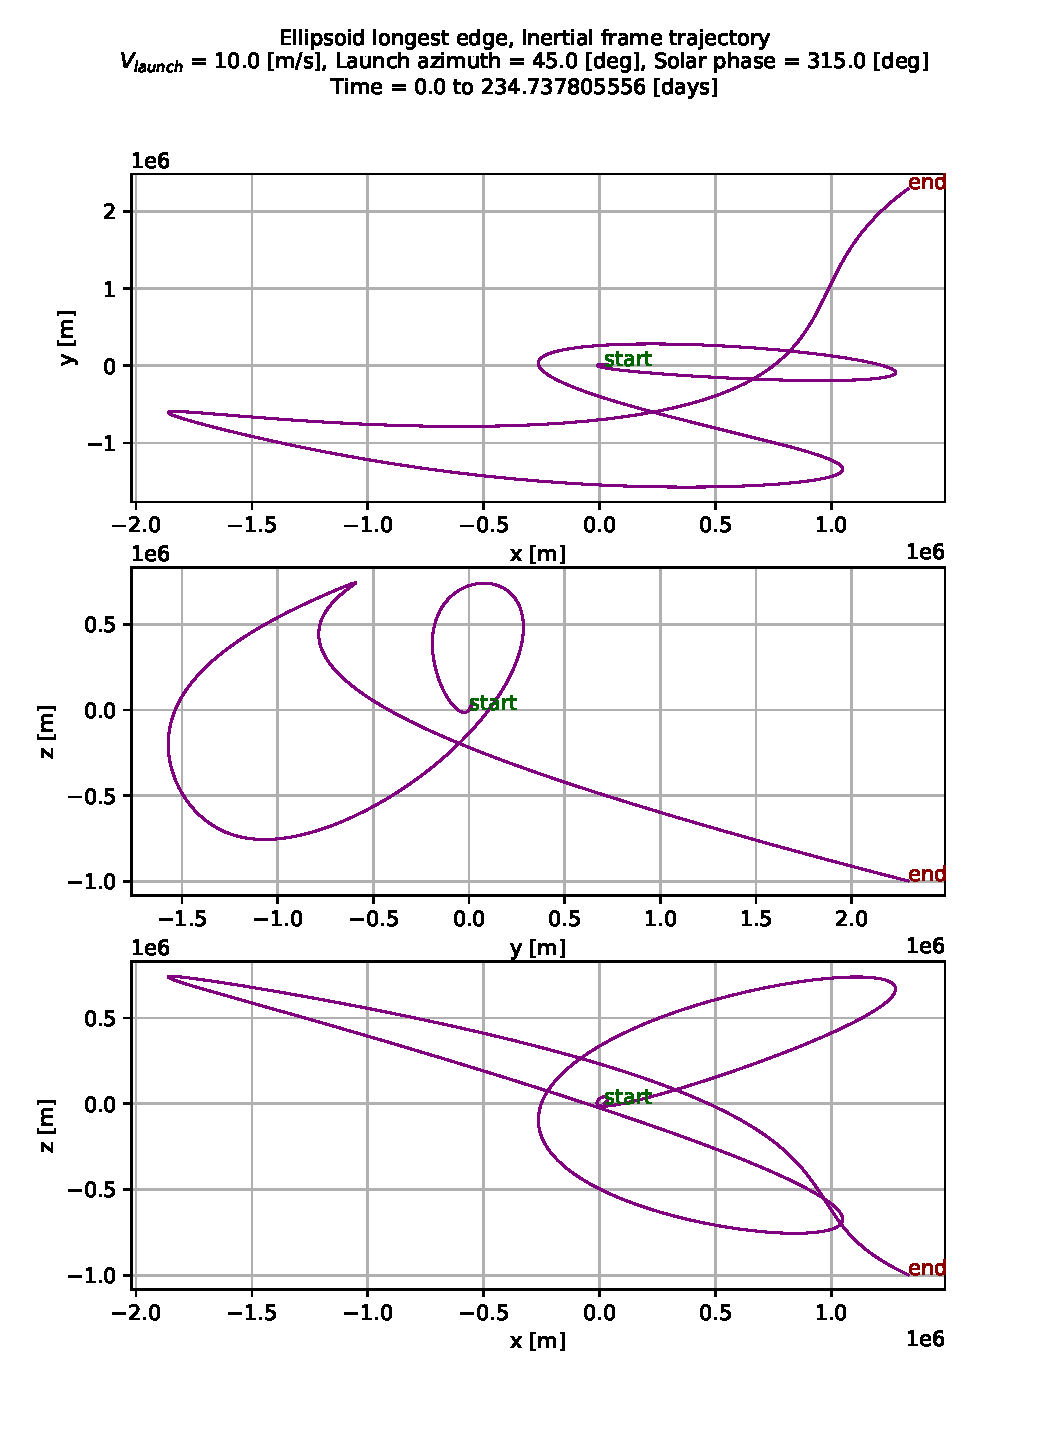
\includegraphics[width=\linewidth, height=\textheight, keepaspectratio=true]{longest_edge_perturbations/3.2Density_1cmSize/10ms_45Azimuth_315SolarPhase/noSTBE_2d_trajectory_inertialFrame.pdf}
\caption{2D trajectory of particle for same initial conditions as that of capture case 5 in \Cref{tab:LoGSP_1_capture} except that only \gls{SRP} was included in this simulation. Particle code LoGSP-1.}
\label{fig:LoGSP_1_capture_case_5_2d_inertialTrajectory_noSTBE}
\end{figure}
\FloatBarrier
%%%
%%%
\begin{figure}[htb]
\centering
\captionsetup{justification=centering}
\subfloat[]{
    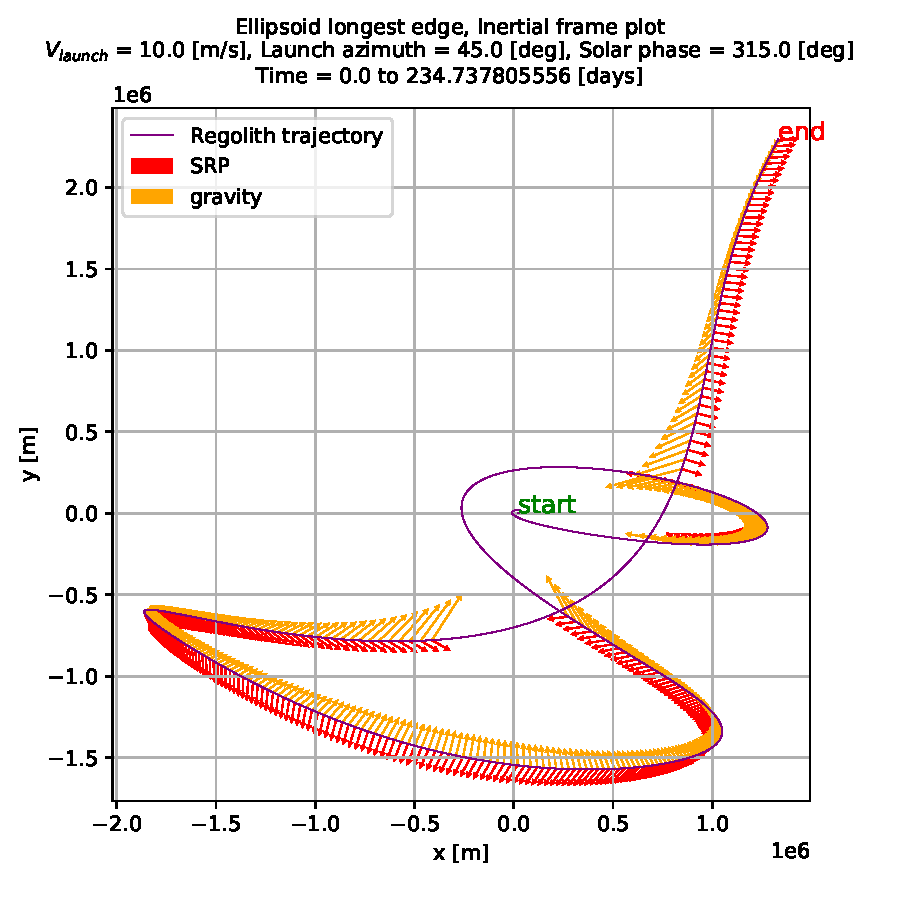
\includegraphics[width=\linewidth, height=0.45\textheight, keepaspectratio=true]{longest_edge_perturbations/3.2Density_1cmSize/10ms_45Azimuth_315SolarPhase/noSTBE_srp_gravity_vectors_inertialFrame.pdf}
    \label{fig:LoGSP_1_capture_case_5_2d_SRP_and_gravity_vector_noSTBE_inertialFrame}
}

\subfloat[]{
    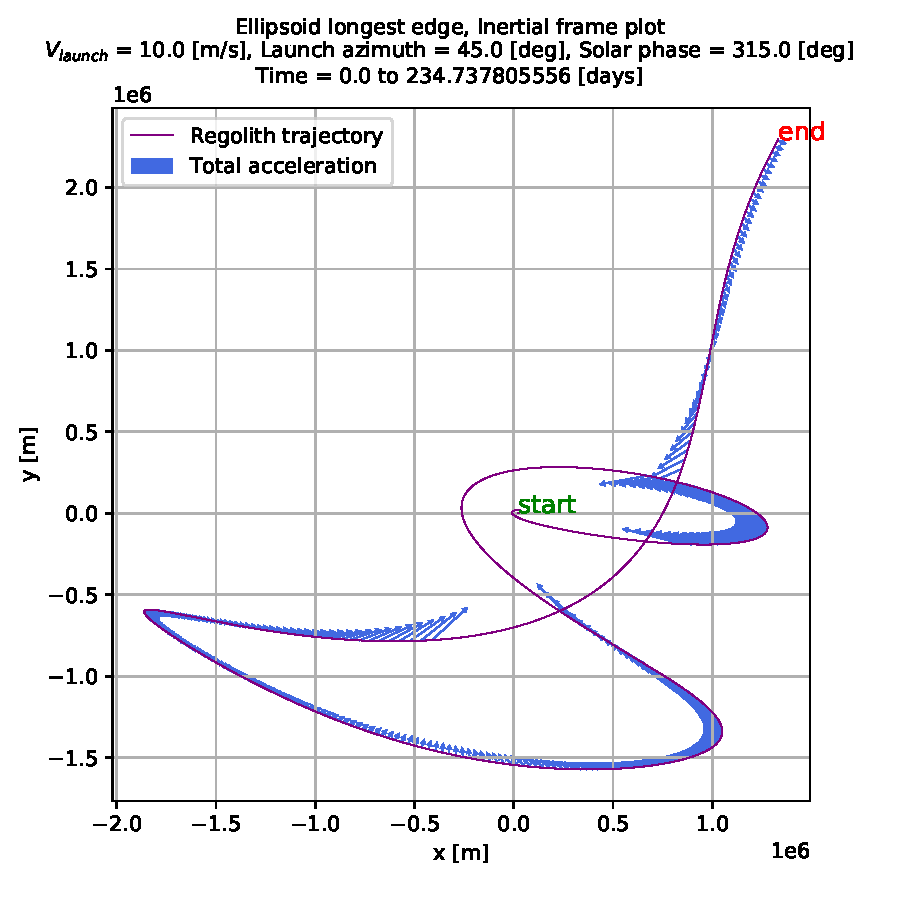
\includegraphics[width=\linewidth, height=0.45\textheight, keepaspectratio=true]{longest_edge_perturbations/3.2Density_1cmSize/10ms_45Azimuth_315SolarPhase/noSTBE_total_acceleration_inertialFrame.pdf}
    \label{fig:LoGSP_1_capture_case_5_2d_totalAcceleration_vector_noSTBE_inertialFrame}
}
\caption{Inertial frame XY plane trajectory for same launch conditions as that of capture case 5 in \Cref{tab:LoGSP_1_capture}: \protect\subref{fig:LoGSP_1_capture_case_5_2d_SRP_and_gravity_vector_noSTBE_inertialFrame} showing direction of \gls{SRP} acceleration and gravitational acceleration \& \protect\subref{fig:LoGSP_1_capture_case_5_2d_totalAcceleration_vector_noSTBE_inertialFrame} showing direction of the net acceleration acting on the particle. Vectors are shown only for those parts of trajectory where acceleration due to \gls{SRP} and gravity have the same order of magnitude. Note that \gls{STBE} perturbation was not part of the simulation here. Particle code LoGSP-1.}
\end{figure}
\FloatBarrier
%%%
When we keep \gls{STBE} but remove \gls{SRP} from our simulations, then the trajectory again leads to an escape situation, only this time its much faster. The 2D inertial frame trajectory is shown in \Cref{fig:LoGSP_1_capture_case_5_2d_inertialTrajectory_noSRP}. The trajectory shows similarity only for a brief moment immediately after launch (notice the small loop after 'start') with the capture case in \Cref{fig:LoGSP_1_capture_case_5_2d_traj_inertialFrame} but soon after the particle is on a trajectory that never comes back around the asteroid. The reason for this is clear and simple if one looks at the direction of acceleration due to gravity and \gls{STBE} in \Cref{fig:LoGSP_1_capture_case_5_2d_STBE_and_gravity_vector_noSRP_inertialFrame} and their net effect in \Cref{fig:LoGSP_1_capture_case_5_2d_totalAcceleration_vector_noSRP_inertialFrame}. Initially, from the point when we show these vectors, we know that the magnitude of \gls{STBE} acceleration is 1.0 order of magnitude smaller than the gravitational acceleration (see \Cref{fig:LoGSP_1_capture_case_5_2d_acceleration_magnitudes_noSRP}) and even then the direction of the net acceleration vector is such that the trajectory can not loop around the asteroid. The \gls{STBE} magnitude increases soon enough to the same order as that of gravitational acceleration and the net acceleration vector direction never points towards the asteroid which eventually causes the particle to escape. However, the point where the magnitude curves of \gls{STBE} and gravitational acceleration cross is not the point where the escape occurs as is evident from the plot for total energy and eccentricity in \Cref{fig:LoGSP_1_capture_case_5_eccentricity_energy_noSRP}.

From this analysis, we can say that effect of removing \gls{SRP} from simulations had a much drastic effect than removing just the \gls{STBE}. Both cases lead to an escape situation and the combined effect of both the perturbations leads to a capture orbit, for the same launch conditions and initial Solar phase angle. The behavior of the trajectory, in all cases, can be easily understood by looking at the direction of the net acceleration vector, especially when the particle is far away from the asteroid because it tells us exactly, how by adding perturbations, the motion of the particle is affected and not just in terms of its final fate but even in terms of changing its orbital direction.
%%%
\begin{figure}[htb]
\centering
\captionsetup{justification=centering}
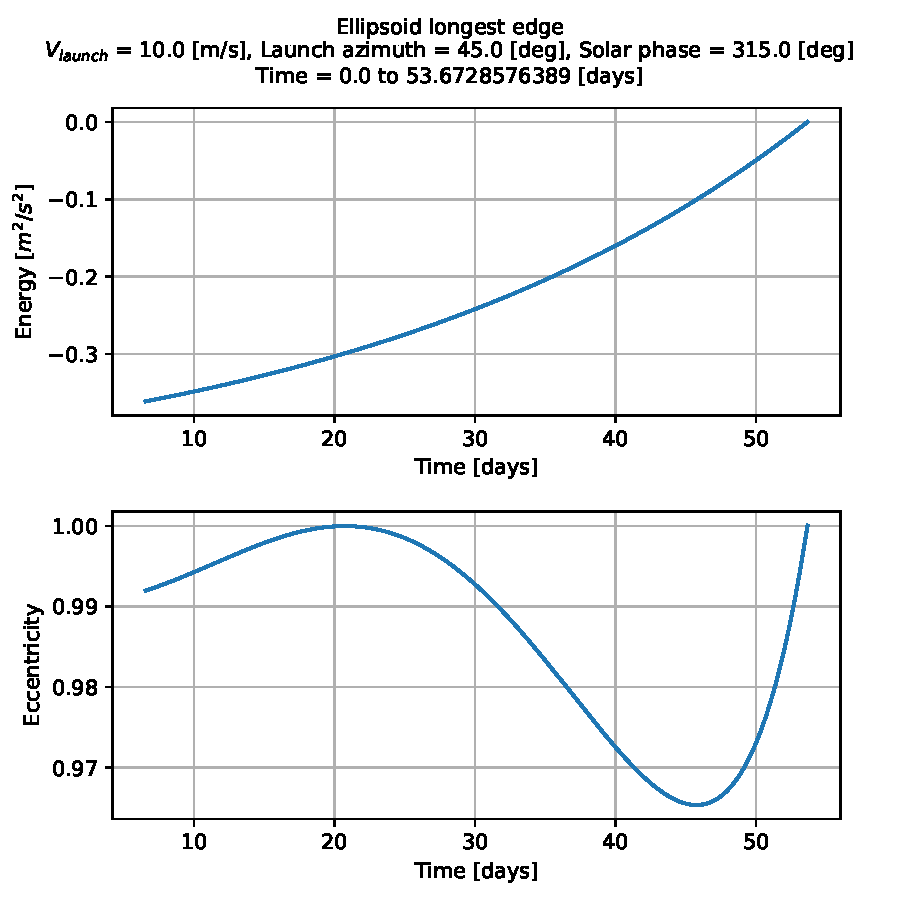
\includegraphics[width=\linewidth, height=0.45\textheight, keepaspectratio=true]{longest_edge_perturbations/3.2Density_1cmSize/10ms_45Azimuth_315SolarPhase/noSRP_eccentricity_energy.pdf}
\caption{Evolution of total energy of the particle and its orbital eccentricity. Particle has the same initial conditions as that of capture case 5 in \Cref{tab:LoGSP_1_capture} except that only \gls{STBE} was included in this simulation. The range of data points plotted is the same as that in \Cref{fig:LoGSP_1_capture_case_5_2d_noSRP_accelerationVectorPlot_inertialFrame}. Particle code LoGSP-1.}
\label{fig:LoGSP_1_capture_case_5_eccentricity_energy_noSRP}
\end{figure}
\FloatBarrier
%%%
%%%
\begin{figure}[htb]
\centering
\captionsetup{justification=centering}
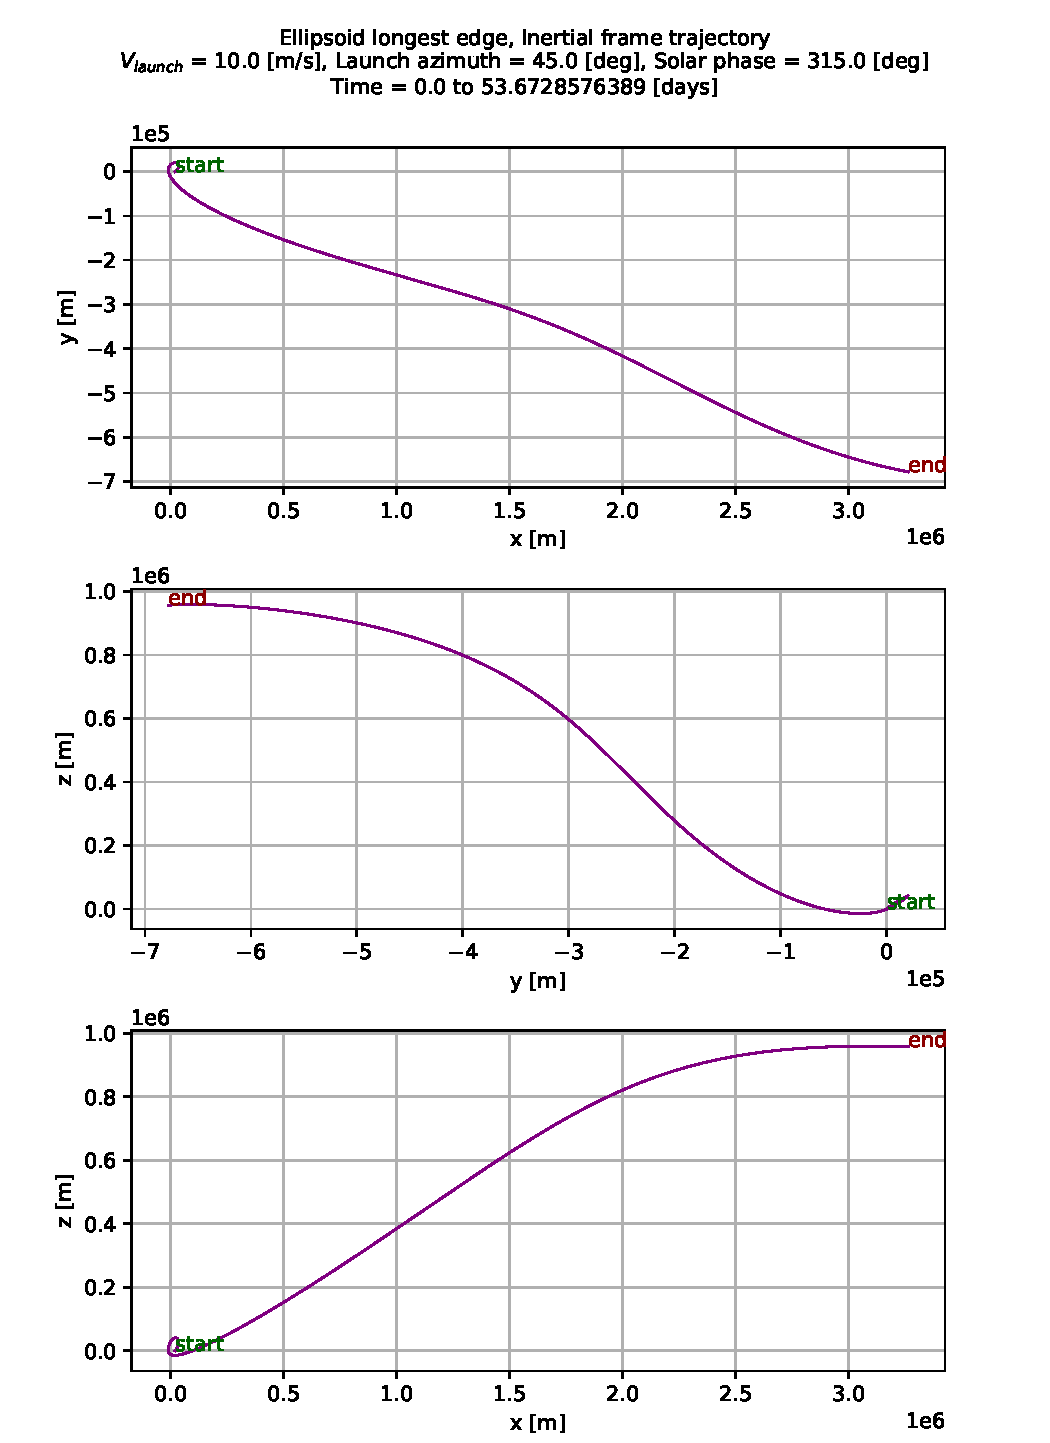
\includegraphics[width=\linewidth, height=\textheight, keepaspectratio=true]{longest_edge_perturbations/3.2Density_1cmSize/10ms_45Azimuth_315SolarPhase/noSRP_2d_trajectory_inertialFrame.pdf}
\caption{2D trajectory of particle for same initial conditions as that of capture case 5 in \Cref{tab:LoGSP_1_capture} except that only \gls{STBE} was included in this simulation. Particle code LoGSP-1.}
\label{fig:LoGSP_1_capture_case_5_2d_inertialTrajectory_noSRP}
\end{figure}
\FloatBarrier
%%%
%%%
\begin{figure}[htb]
\centering
\captionsetup{justification=centering}
\subfloat[]{
    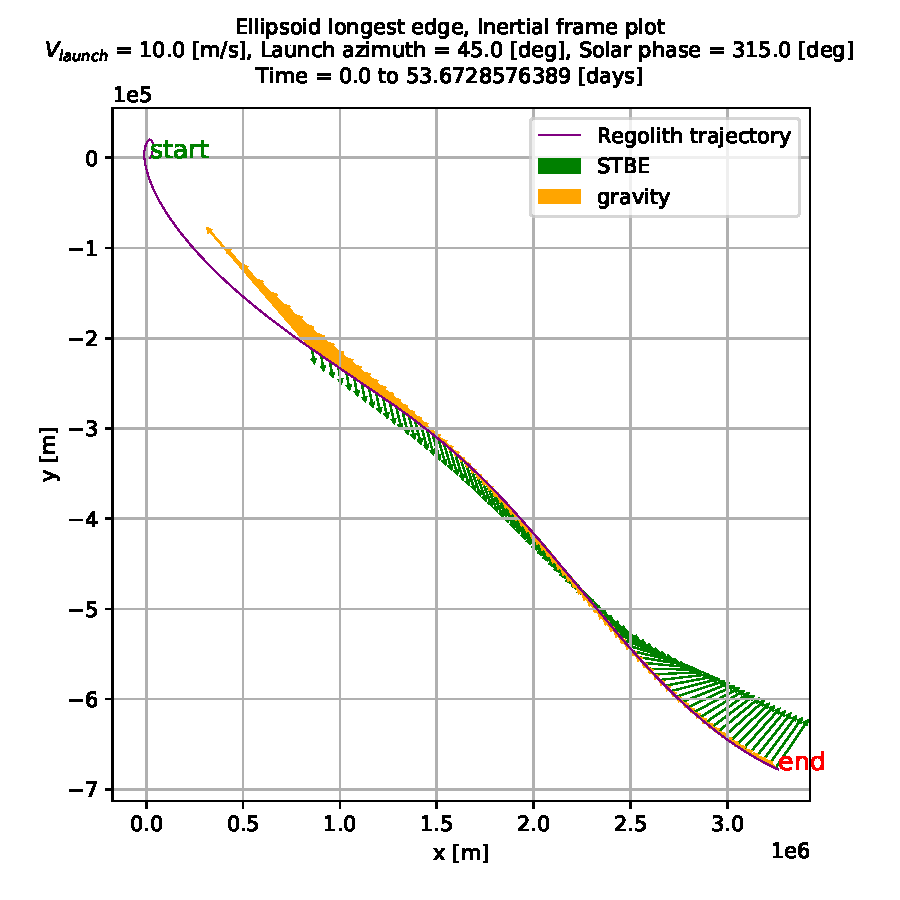
\includegraphics[width=\linewidth, height=0.45\textheight, keepaspectratio=true]{longest_edge_perturbations/3.2Density_1cmSize/10ms_45Azimuth_315SolarPhase/noSRP_stbe_gravity_vectors_inertialFrame.pdf}
    \label{fig:LoGSP_1_capture_case_5_2d_STBE_and_gravity_vector_noSRP_inertialFrame}
}

\subfloat[]{
    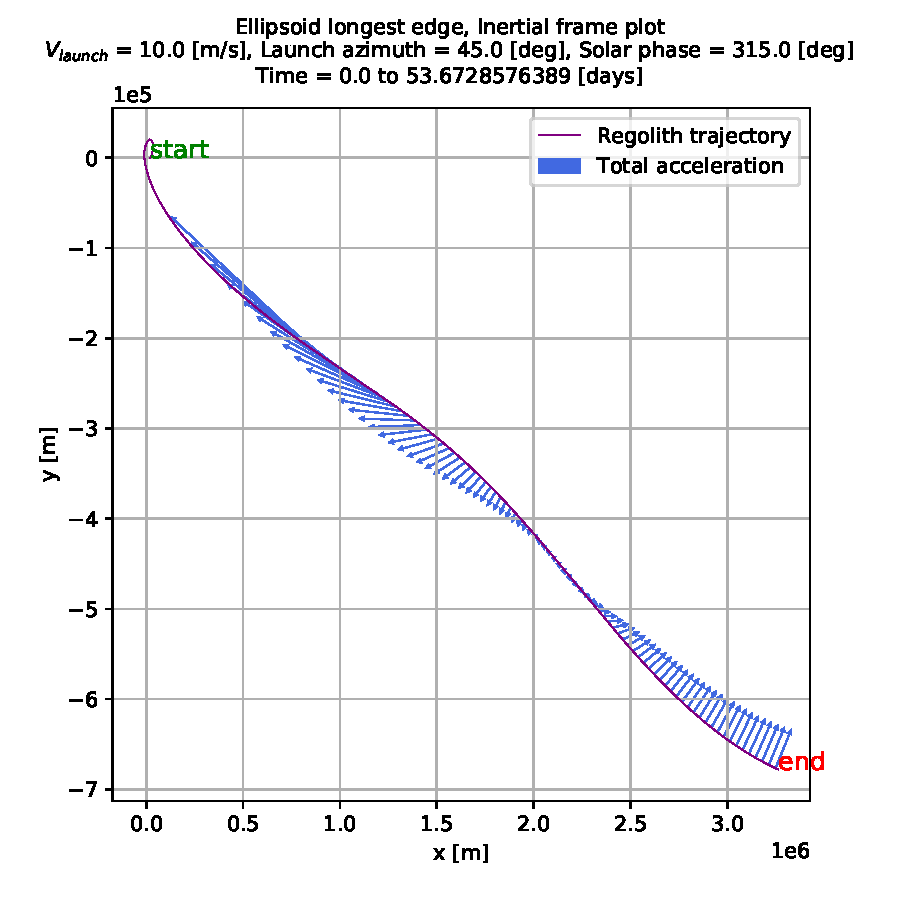
\includegraphics[width=\linewidth, height=0.45\textheight, keepaspectratio=true]{longest_edge_perturbations/3.2Density_1cmSize/10ms_45Azimuth_315SolarPhase/noSRP_total_acceleration_inertialFrame.pdf}
    \label{fig:LoGSP_1_capture_case_5_2d_totalAcceleration_vector_noSRP_inertialFrame}
}
\caption{Inertial frame XY plane trajectory for same launch conditions as that of capture case 5 in \Cref{tab:LoGSP_1_capture}: \protect\subref{fig:LoGSP_1_capture_case_5_2d_STBE_and_gravity_vector_noSRP_inertialFrame} showing direction of \gls{STBE} acceleration and gravitational acceleration \& \protect\subref{fig:LoGSP_1_capture_case_5_2d_totalAcceleration_vector_noSRP_inertialFrame} showing direction of the net acceleration acting on the particle. Vectors are shown only for those parts of trajectory where acceleration due to \gls{STBE} is equal to gravitational acceleration or smaller than it by 1.0 order of magnitude. Note that \gls{SRP} perturbation was not part of the simulation here. Particle code LoGSP-1.}
\label{fig:LoGSP_1_capture_case_5_2d_noSRP_accelerationVectorPlot_inertialFrame}
\end{figure}
\FloatBarrier
%%%
%%%
\begin{figure}[htb]
\centering
\captionsetup{justification=centering}
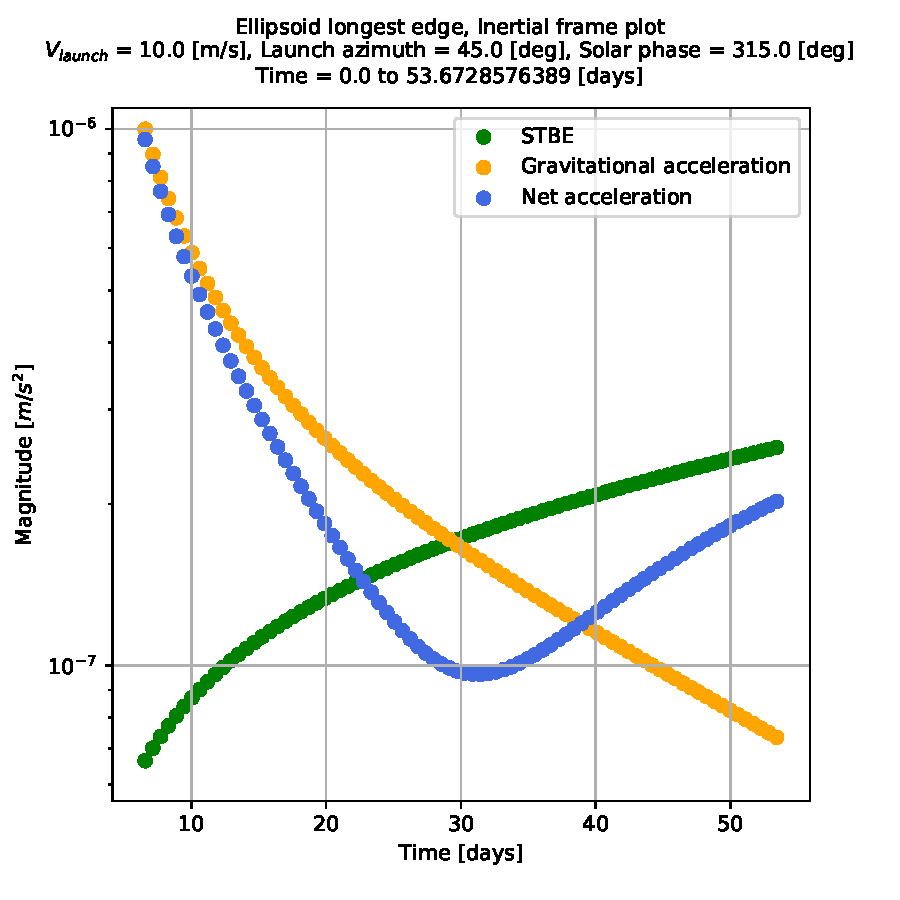
\includegraphics[width=\linewidth, height=0.50\textheight, keepaspectratio=true]{longest_edge_perturbations/3.2Density_1cmSize/10ms_45Azimuth_315SolarPhase/noSRP_acceleration_magnitudes.pdf}
\caption{Magnitudes of acceleration due to gravity, \gls{STBE} and the net effect of the two for the corresponding vectors as shown in \Cref{fig:LoGSP_1_capture_case_5_2d_noSRP_accelerationVectorPlot_inertialFrame}. Particle code LoGSP-1.}
\label{fig:LoGSP_1_capture_case_5_2d_acceleration_magnitudes_noSRP}
\end{figure}
\FloatBarrier
%%%

\Cref{fig:LoGSP_1_capture_case_8_3d_traj_inertialFrame_differnetViews} shows the 3D trajectory for completely different launch conditions (see capture case 8 in \Cref{tab:LoGSP_1_capture}). The 3D trajectory as viewed from the asteroid centric body fixed frame is shown in \Cref{fig:LoGSP_1_capture_case_8_3d_trajectory}. The 2D trajectory projections for the same, in inertial and body fixed frames, are shown in \Cref{fig:LoGSP_1_capture_case_8_2d_traj_inertialFrame} and \Cref{fig:LoGSP_1_capture_case_8_2d_traj_bodyFrame} respectively. Just like in the previous case, we see from the animation (see \Cref{fig:LoGSP_1_capture_case_8_2d_trajectory_animation}) and the 3D trajectory for current launch conditions, that the particle direction of motion is reversed twice in its course. These two locations are marked by numbers 1 and 2 in \Cref{fig:LoGSP_1_capture_case_8_2d_traj_inertialFrame}. At location number 1 we see that the motion changes from anti-clockwise to clockwise direction in the XY plane. The case for location number 2 is exactly the opposite. If we look at \Cref{fig:LoGSP_1_capture_case_8_2d_trajectory_totalPerturbationVectors}, the change in direction of motion is consistent with the direction in which the net perturbing force is acting. Ultimately, when we look at the net acceleration acting on the particle in \Cref{fig:LoGSP_1_capture_case_8_2d_totalAccelerationVector}, we can understand how exactly the particle would orbit around the asteroid. The net force, gravitational and perturbations combined, act in a direction such that the particle is forced to change its orbital motion direction at the two locations previously explained. The acceleration vectors in \Cref{fig:LoGSP_1_capture_case_8_2d_trajectory_perturbationVectors,fig:LoGSP_1_capture_case_8_2d_trajectory_totalPerturbations_and_gravity_vectors,fig:LoGSP_1_capture_case_8_2d_totalAccelerationVector} are plotted for points along the trajectory where the magnitude of acceleration due to \gls{SRP} is of the same order of magnitude as the gravitational acceleration. Again, the magnitude of \gls{STBE} is 1.0 order of magnitude smaller than the gravitational acceleration for the same data points along the trajectory.
%%%
\begin{figure}[htb]
\centering
\captionsetup{justification=centering}
% another option for includegraphics - keepaspectratio
\subfloat[]{
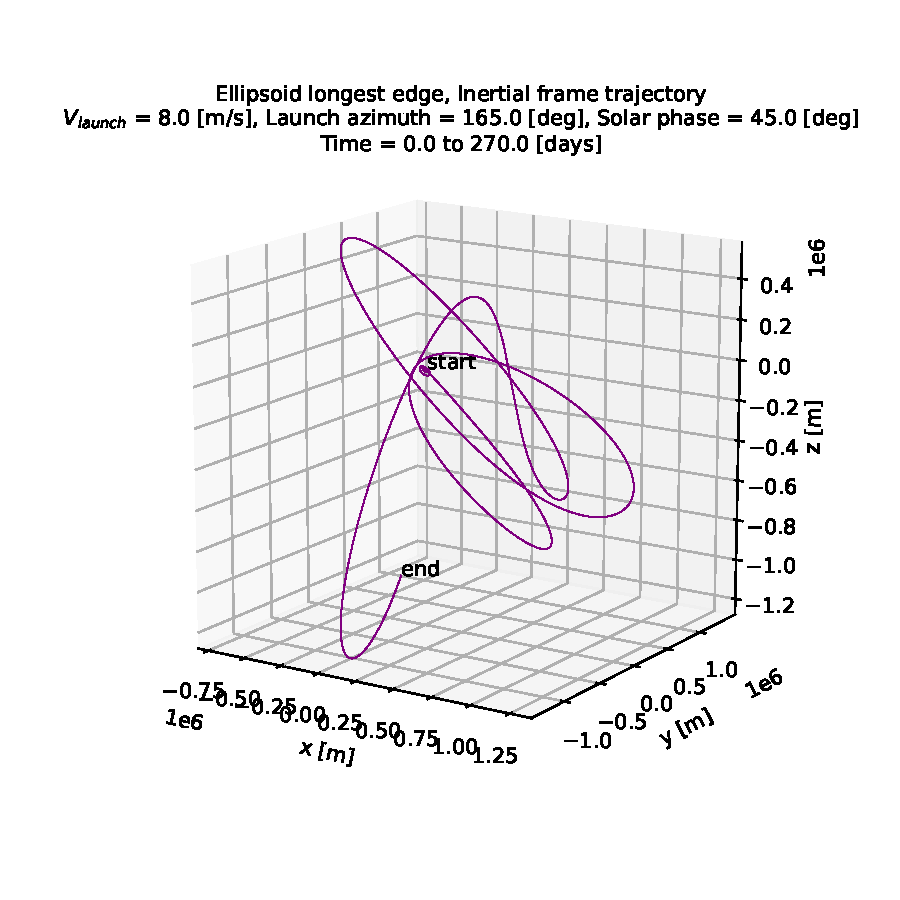
\includegraphics[width=\textwidth, height=0.5\textheight, keepaspectratio=true]{longest_edge_perturbations/3.2Density_1cmSize/3dTrajectory_8ms_165Azimuth_45solarPhase_inertialFrame_View1.pdf}
}

\subfloat[]{
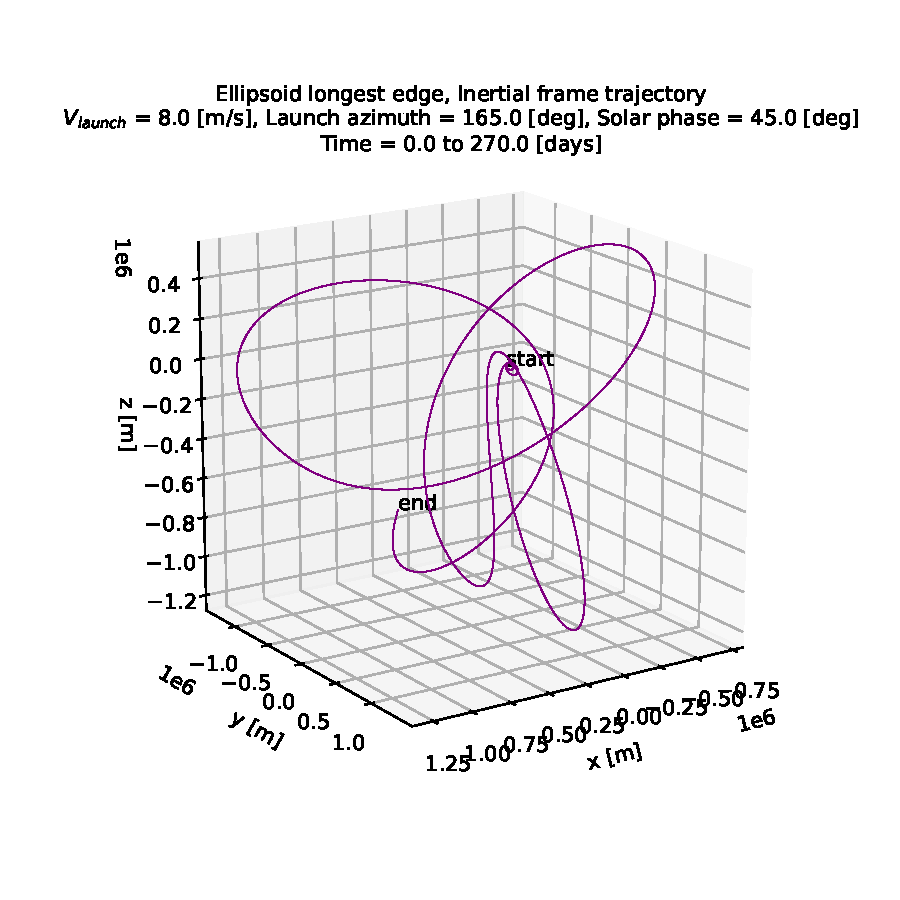
\includegraphics[width=\textwidth, height=0.5\textheight, keepaspectratio=true]{longest_edge_perturbations/3.2Density_1cmSize/3dTrajectory_8ms_165Azimuth_45solarPhase_inertialFrame_View2.pdf}
}
\caption{3D inertial frame trajectory of capture regolith for case number 8 in \Cref{tab:LoGSP_1_capture} from two different viewing angles. Particle code LoGSP-1.}
\label{fig:LoGSP_1_capture_case_8_3d_traj_inertialFrame_differnetViews}
\end{figure}
\FloatBarrier
%%%
%%%
\begin{figure}[htb]
\centering
\captionsetup{justification=centering}
% another option for includegraphics - keepaspectratio
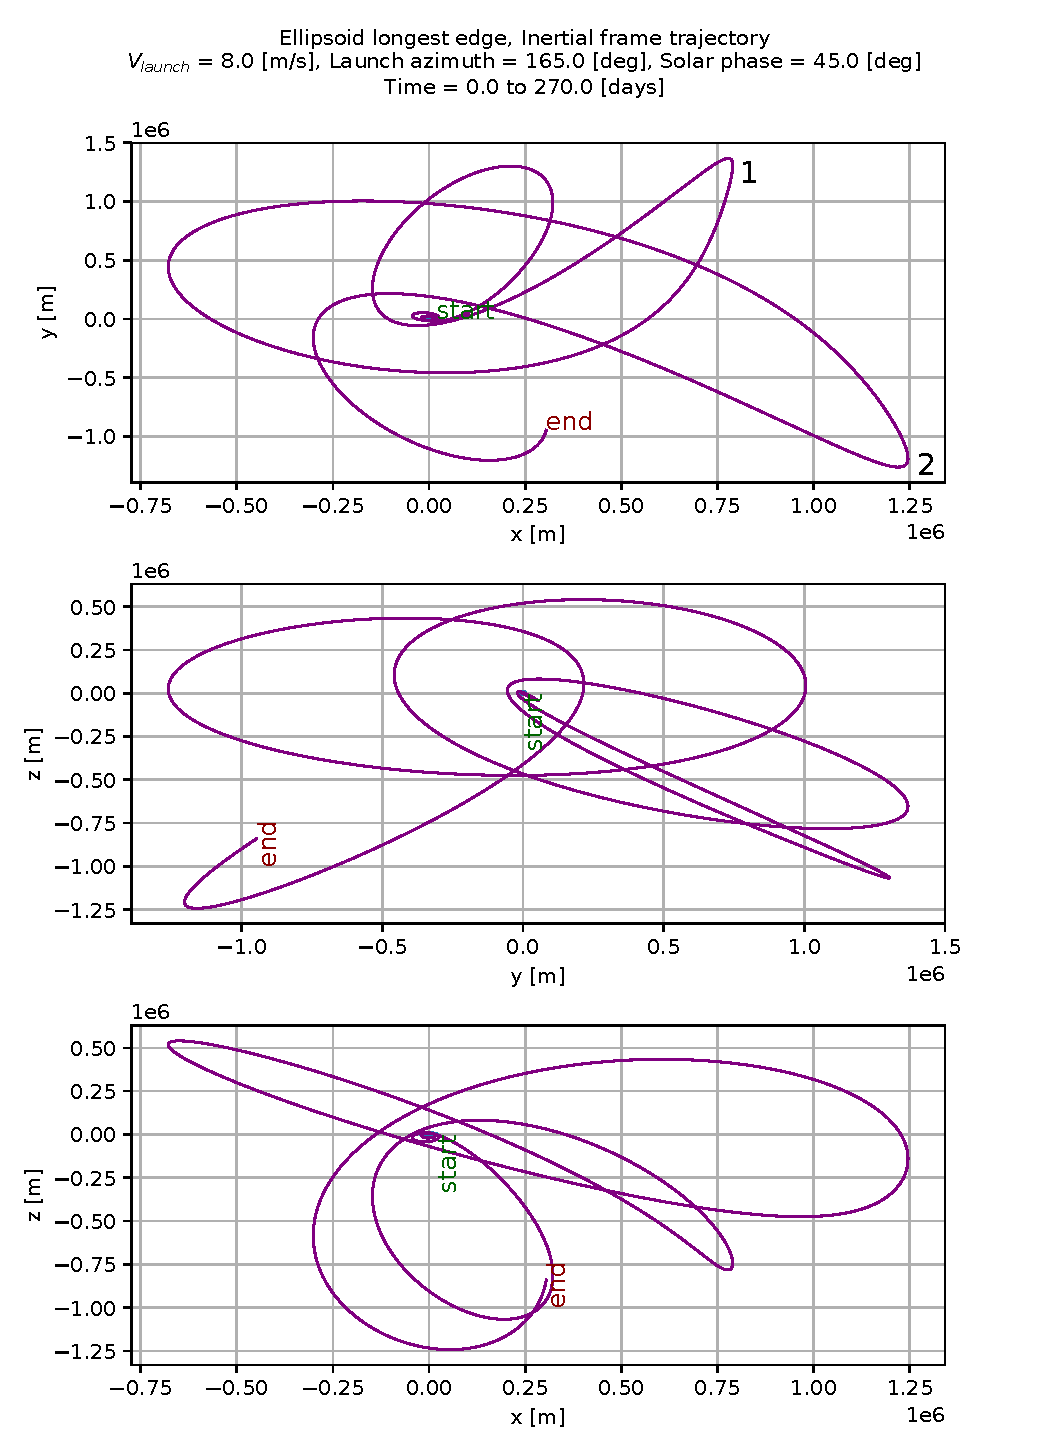
\includegraphics[width=\textwidth, height=\textheight]{longest_edge_perturbations/3.2Density_1cmSize/2dTrajectory_8ms_165Azimuth_45solarPhase_inertialFrame_edit.pdf}
\caption{2D inertial frame trajectory of capture regolith for case number 8 in \Cref{tab:LoGSP_1_capture}. Particle code LoGSP-1.}
\label{fig:LoGSP_1_capture_case_8_2d_traj_inertialFrame}
\end{figure}
\FloatBarrier
%%%
%%%
\begin{figure}[htb]
\centering
\captionsetup{justification=centering}
% another option for includegraphics - keepaspectratio
\subfloat[]{
    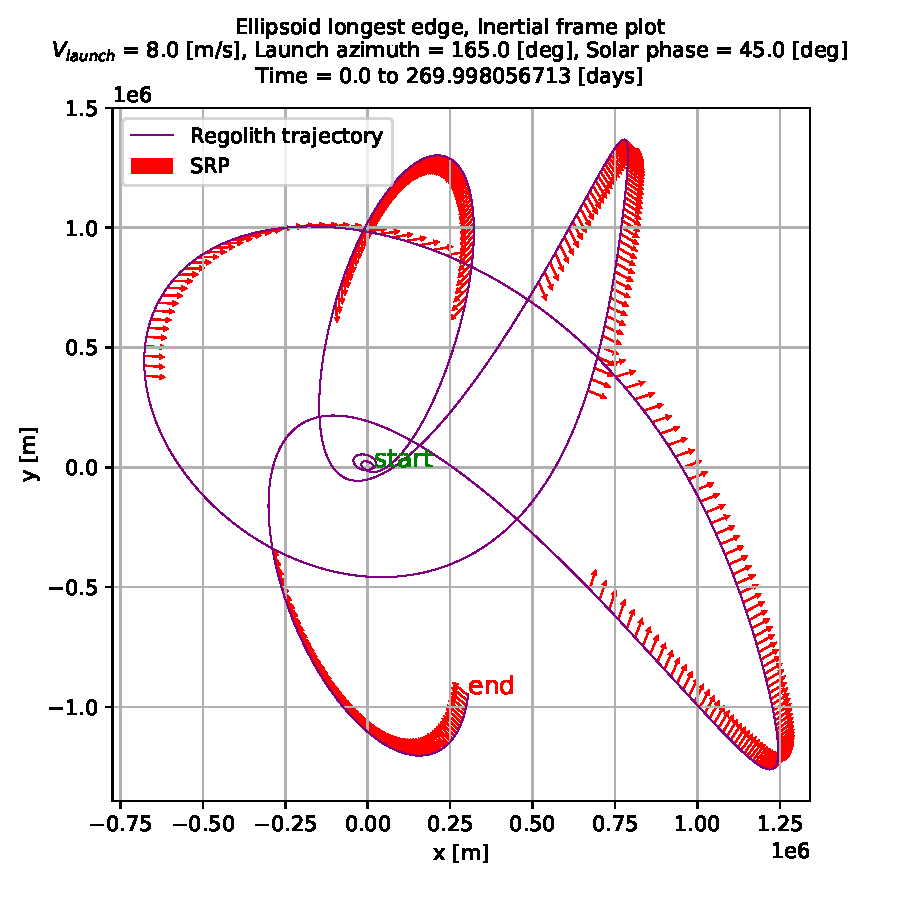
\includegraphics[width=\textwidth, height=0.45\textheight, keepaspectratio=true]{longest_edge_perturbations/3.2Density_1cmSize/8ms_165Azimuth_45SolarPhase/srp_vectors.pdf}
    \label{fig:LoGSP_1_capture_case_8_2d_trajectory_srp_vectors}
}

\subfloat[]{
    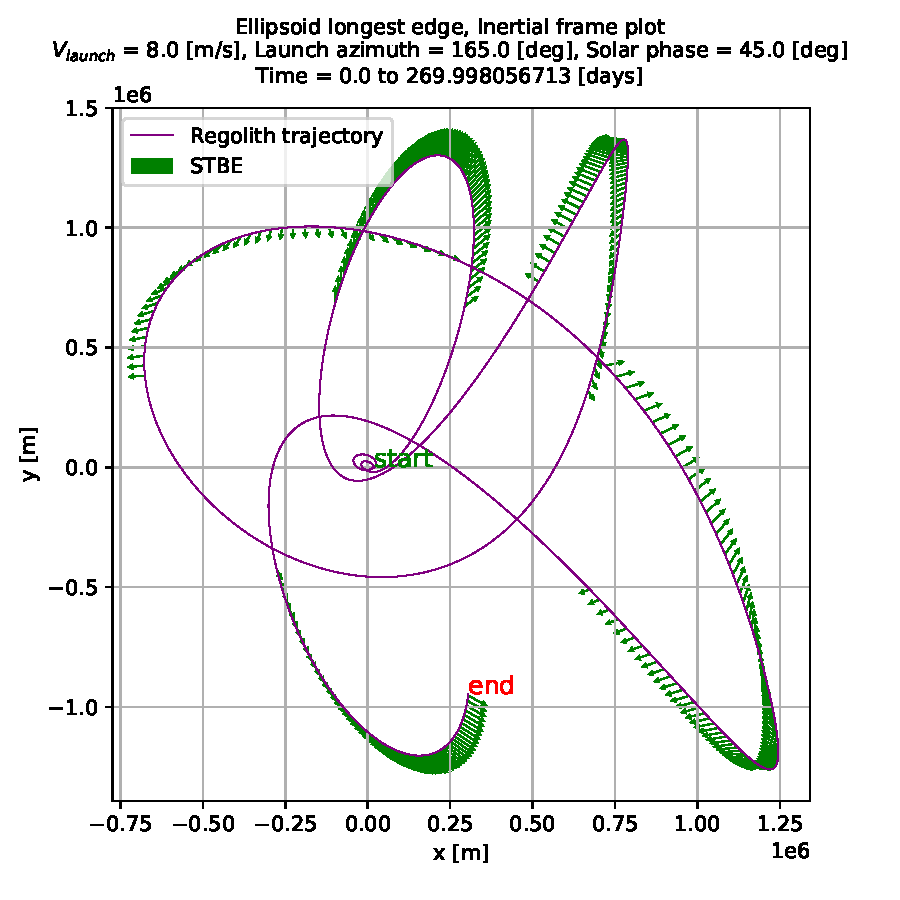
\includegraphics[width=\textwidth, height=0.45\textheight, keepaspectratio=true]{longest_edge_perturbations/3.2Density_1cmSize/8ms_165Azimuth_45SolarPhase/stbe_vectors.pdf}
    \label{fig:LoGSP_1_capture_case_8_2d_trajectory_stbe_vectors}
}
\caption{2D trajectory of capture regolith for case number 8 in \Cref{tab:LoGSP_1_capture} with direction of \gls{SRP} and \gls{STBE} perturbation vectors. Note that the vectors are shown only for those parts of the trajectory where the \gls{SRP} magnitude is of the same order as that of the asteroid's gravitational acceleration. For those very same points along the trajectory, the magnitude of the \gls{STBE} is always 1.0 order of magnitude smaller than the gravitational acceleration. Particle code LoGSP-1.}
\label{fig:LoGSP_1_capture_case_8_2d_trajectory_perturbationVectors}
\end{figure}
\FloatBarrier
%%%
%%%
\begin{figure}[htb]
\centering
\captionsetup{justification=centering}
\subfloat[]{
    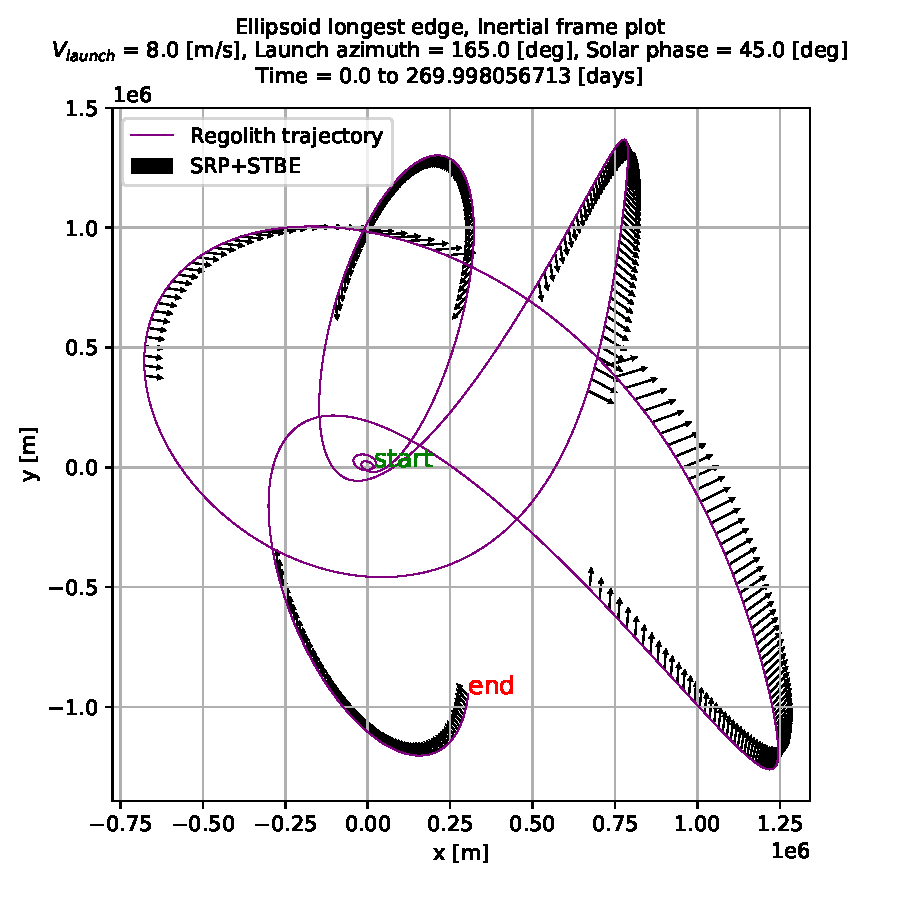
\includegraphics[width=\linewidth, height=0.45\textheight, keepaspectratio=true]{longest_edge_perturbations/3.2Density_1cmSize/8ms_165Azimuth_45SolarPhase/netPerturbations_vectors.pdf}
    \label{fig:LoGSP_1_capture_case_8_2d_trajectory_totalPerturbationVectors}
}

\subfloat[]
{
    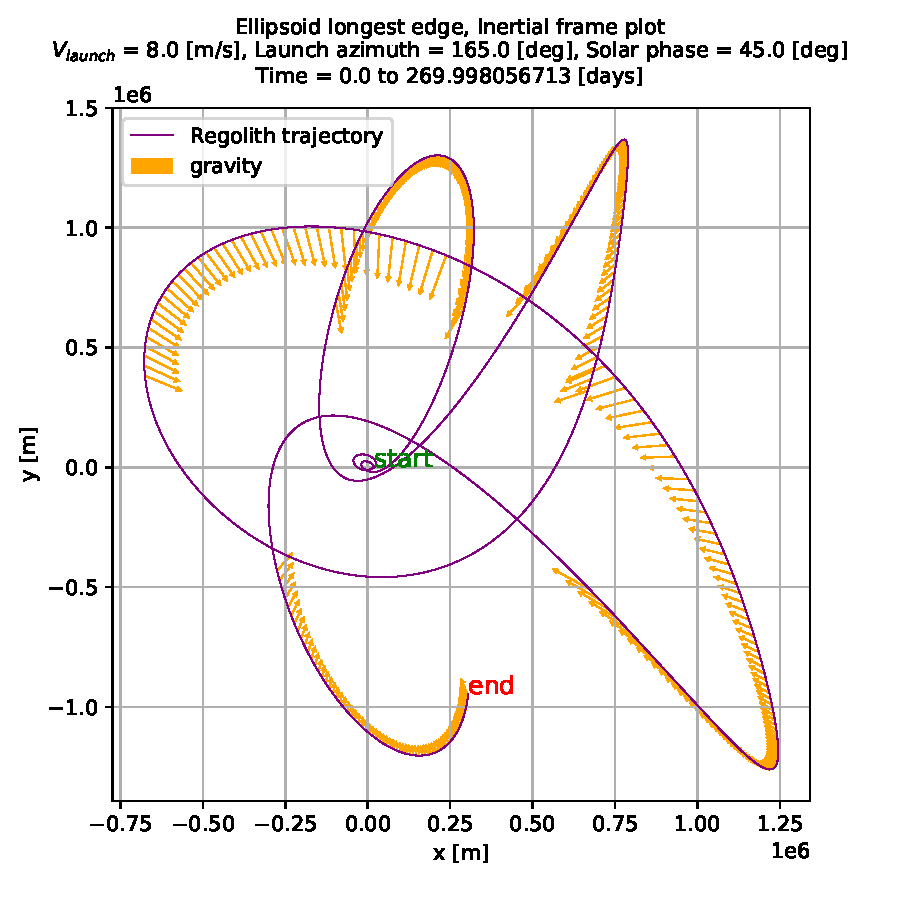
\includegraphics[width=\linewidth, height=0.45\textheight, keepaspectratio=true]{longest_edge_perturbations/3.2Density_1cmSize/8ms_165Azimuth_45SolarPhase/gravity_vectors.pdf}
    \label{fig:LoGSP_1_capture_case_8_2d_trajectory_gravityVector}
}
\caption{2D trajectory of capture regolith for case number 8 in \Cref{tab:LoGSP_1_capture} with direction of the sum total of \gls{SRP} and \gls{STBE} perturbation vectors, and the direction of the gravitational acceleration vector for the same data points. Note that the vectors are shown only for those parts of the trajectory where the \gls{SRP} magnitude is of the same order as that of the asteroid's gravitational acceleration. For those very same points along the trajectory, the magnitude of the \gls{STBE} is always 1.0 order of magnitude smaller than the gravitational acceleration. Particle code LoGSP-1.}
\label{fig:LoGSP_1_capture_case_8_2d_trajectory_totalPerturbations_and_gravity_vectors}
\end{figure}
\FloatBarrier
%%%
%%%
\begin{figure}[htb]
\centering
\captionsetup{justification=centering}
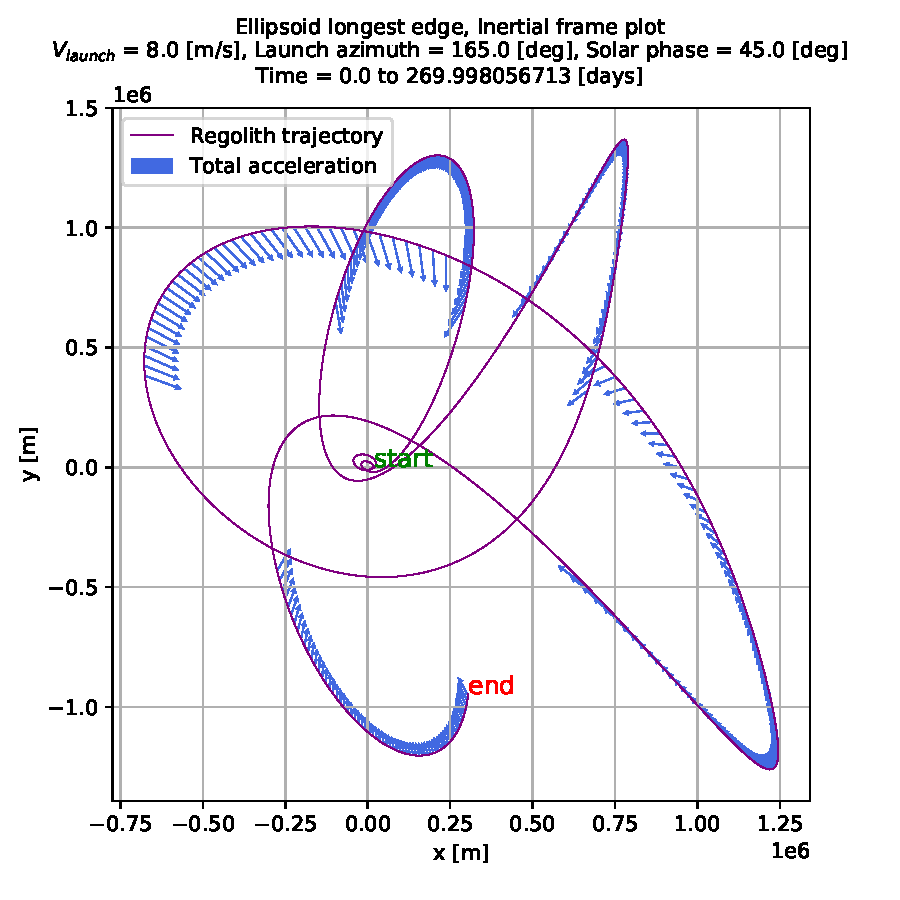
\includegraphics[width=\linewidth, height=0.45\textheight, keepaspectratio=true]{longest_edge_perturbations/3.2Density_1cmSize/8ms_165Azimuth_45SolarPhase/netAcceleration_vectors.pdf}
\caption{2D trajectory of capture regolith for case number 8 in \Cref{tab:LoGSP_1_capture} with direction of the net acceleration vector. Note that the vectors are shown only for those parts of the trajectory where the \gls{SRP} magnitude is of the same order as that of the asteroid's gravitational acceleration. For those very same points along the trajectory, the magnitude of the \gls{STBE} is always 1.0 order of magnitude smaller than the gravitational acceleration. Particle code LoGSP-1.}
\label{fig:LoGSP_1_capture_case_8_2d_totalAccelerationVector}
\end{figure}
\FloatBarrier
%%%
%%%
\begin{figure}[htb]
\centering
\captionsetup{justification=centering}
% another option for includegraphics - keepaspectratio

\includegraphics[scale=0.25]{longest_edge_perturbations/3.2Density_1cmSize/qrcode_8ms_165Azimuth_45SolarPhase.png}
\caption{2D trajectory animation (XY Plane) of capture regolith for case number 8 in \Cref{tab:LoGSP_1_capture}. Particle code LoGSP-1. Scan the QR code to view the animation or use the following web-link: \url{https://youtu.be/CceYRlNvAiM}}
\label{fig:LoGSP_1_capture_case_8_2d_trajectory_animation}
\end{figure}
\FloatBarrier
%%%

%%%%%%%%%%%%%% 2nd edit needed %%%%%%%%%%%%%%%%%%%%%%%%%%%%%%%

We saw in the analysis of capture case number 5 for particle LoGSP-1 that both \gls{SRP} and \gls{STBE} were necessary for getting that specific capture trajectory and removal of either of the perturbations resulted in a different final fate for the same particle. The next analysis that we present now, will tell us about how a capture scenario occurs, relative to a situation when all perturbations are removed, for the same initial launch conditions in both cases. We do the analysis for capture case number 8 from \Cref{tab:LoGSP_1_capture}. \Cref{fig:LoGSP_1_capture_case_8_2d_trajectory_comparative_inertialFrame} shows two different trajectories for the particle launched with the same initial conditions. The one shown in dotted line is for the case when Solar perturbations were omitted from the simulation, which eventually results in the particle escaping the asteroid after 1.4 [days]. The one in the solid line shows the capture trajectory (actually a section of the entire capture trajectory as seen in \Cref{fig:LoGSP_1_capture_case_8_2d_traj_inertialFrame}) when Solar perturbations were included in the simulation. Note that we show the perturbed trajectory (capture case) for the same amount of time (1.4 [days] instead of 270.0 [days]) as taken by the unperturbed trajectory (escape case) to be able to do a one-to-one comparison. The arrows plotted along this trajectory indicate the direction of the net perturbing acceleration due to \gls{SRP} and \gls{STBE}. \Cref{fig:LoGSP_1_capture_case_8_2d_trajectory_comparative_animation} directs to an animation for both the unperturbed and perturbed trajectory.
%%%
\begin{figure}[htb]
\centering
\captionsetup{justification=centering}
% another option for includegraphics - keepaspectratio

\includegraphics[scale=0.25]{longest_edge_perturbations/3.2Density_1cmSize/qrcode_comparative_8ms_165Azimuth_45SolarPhase.png}
\caption{2D trajectory animation (XY Plane) of capture regolith for case number 8 in \Cref{tab:LoGSP_1_capture}, compared with that of its unperturbed counterpart. Particle code LoGSP-1. Scan the QR code to view the animation or use the following web-link: \url{https://youtu.be/CdFKKR3UDJ0}}
\label{fig:LoGSP_1_capture_case_8_2d_trajectory_comparative_animation}
\end{figure}
\FloatBarrier
%%%
From the animation we can see that even as the particle has just been lofted from the surface of the asteroid, there are very subtle and minute differences in the range to the particle and its velocity, between the perturbed and unperturbed trajectory. The first visible difference between the two trajectories becomes noticeable at point \textit{"A"} in \Cref{fig:LoGSP_1_capture_case_8_2d_trajectory_comparative_inertialFrame}. It is easy to deduce the change in the perturbed trajectory from the direction of the net perturbing acceleration up until this point. The same point \textit{"A"} is also marked in \Cref{fig:LoGSP_1_capture_case_8_comparative_total_energy}. It is from this point that we can see noticeable difference between the two trajectories as well as in their corresponding energies. A snippet from the trajectory animation, corresponding to the point \textit{"A"}, is shown in \Cref{fig:LoGSP_1_capture_case_8_2d_comparative_animation_snippet} which highlights the differences in range and velocity of the particles in the two trajectories. Note that in \Cref{fig:LoGSP_1_capture_case_8_2d_comparative_animation_snippet}, the difference in the velocity between the perturbed and unperturbed cases is relatively small, compared to almost 1 [km] of a difference in range of the particles. The latter is significant since the particles have dimensions in the order of [cm]. From point \textit{"A"} onwards these differences continue to grow and only get larger as the trajectory proceeds.

Similarly, at point \textit{"B"} in \Cref{fig:LoGSP_1_capture_case_8_2d_trajectory_comparative_inertialFrame}, we see a much larger difference in the two trajectories. In \Cref{fig:LoGSP_1_capture_case_8_comparative_total_energy}, we see that around point \textit{"B"} both trajectories have a positive energy which quickly comes down to a negative value for the perturbed trajectory, hence keeping it bounded which results in a capture scenario. However, this does not happen for the unperturbed trajectory, leading to an escape scenario. The difference in the state of the two particles at point \textit{"B"} are relatively larger and can be seen in \Cref{fig:LoGSP_1_capture_case_8_2d_comparative_animation_phasingExample}. The differences in the two trajectories, computed in the asteroid centric rotating frame, is shown in \Cref{fig:LoGSP_1_capture_case_8_2d_trajectory_comparative_bodyFrame}. The plot on the bottom shows the trajectory for 1.4 [days] (i.e. until escape for the unperturbed trajectory) as viewed in the rotating frame, and the plot on the right zooms into a small part of this trajectory to show how Solar perturbations are responsible for changing the course of the particle. It is seen with a bit more clarity on how the net perturbation vector pulls the trajectory away from the trace of the unperturbed one.

So what we are seeing here is, that due to the inclusion of perturbations from the Sun, the motion of the particle changed from its unperturbed counterpart. This change was not drastic in terms of the initial shape of the trajectory as seen in \Cref{fig:LoGSP_1_capture_case_8_2d_trajectory_comparative_inertialFrame}. But the change was just enough for the particle to have a different phase with respect to the asteroid, relative to the unperturbed trajectory as seen in \Cref{fig:LoGSP_1_capture_case_8_comparative_animation_snapshots}. By phase, we refer to the location of the particle with respect to a given rotational state of the asteroid. So if two particles are at different locations, at any given epoch and for the same rotational state of the asteroid, they will have different magnitudes of forces acting on them which would ultimately lead to different final outcomes.
%%%
\begin{figure}[htb]
\centering
\captionsetup{justification=centering}
\subfloat[]{
    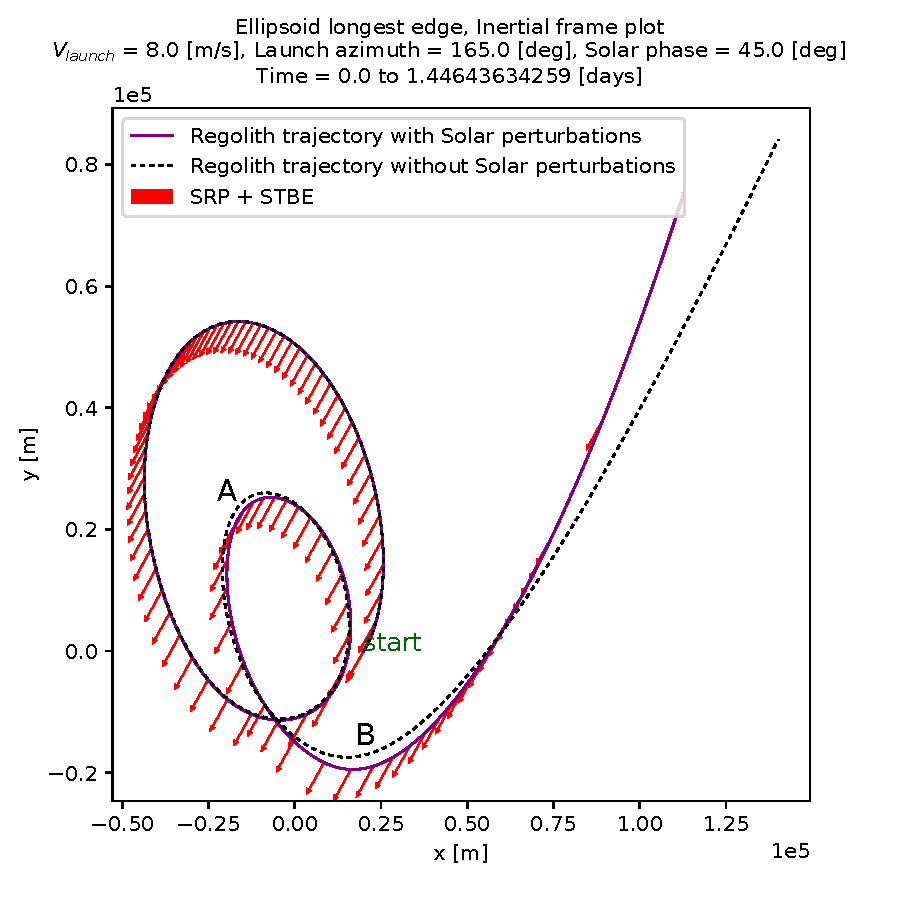
\includegraphics[width=\textwidth, height=0.45\textheight, keepaspectratio=true]{longest_edge_perturbations/3.2Density_1cmSize/8ms_165Azimuth_45SolarPhase/comparative_analysis_allPerturbations_inertialFrame_edit.pdf}
    \label{fig:LoGSP_1_capture_case_8_2d_trajectory_comparative_inertialFrame}
    % \caption{Inertial frame 2D trajectory (XY plane) of capture regolith for case number 8 in \Cref{tab:LoGSP_1_capture} with direction of the net perturbation vector, compared with the trajectory of a particle launched with the same initial conditions but in absence of all Solar perturbations. Vectors are shown after a constant interval of 100 data points. Particle code LoGSP-1.}
}

\subfloat[]{
    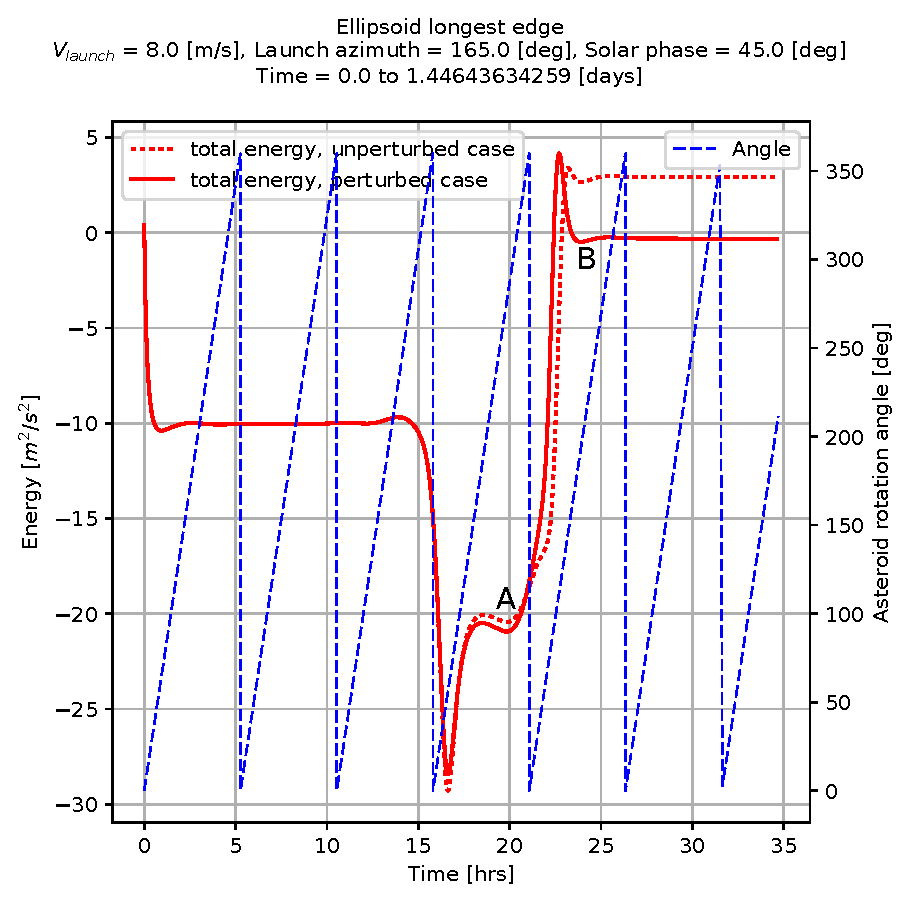
\includegraphics[width=\textwidth, height=0.45\textheight, keepaspectratio=true]{longest_edge_perturbations/3.2Density_1cmSize/8ms_165Azimuth_45SolarPhase/comparative_analysis_total_energy_edit.pdf}
    \label{fig:LoGSP_1_capture_case_8_comparative_total_energy}
    % \caption{Total energy plot for capture case number 8 in \Cref{tab:LoGSP_1_capture} compared with that of a particle launched with the same initial conditions but in absence of all Solar perturbations. Particle code LoGSP-1.}
}
\caption{Comparative analysis of capture case 8 in \Cref{tab:LoGSP_1_capture} with a particle trajectory where the initial conditions are same as the former but the simulation was done without Solar perturbations. \Cref{fig:LoGSP_1_capture_case_8_2d_trajectory_comparative_inertialFrame} compares the XY plane trajectory \& \Cref{fig:LoGSP_1_capture_case_8_comparative_total_energy} compares their total energy. Particle code LoGSP-1.}
\label{fig:LoGSP_1_capture_case_8_comparative analysis_trajectory_and_energy}
\end{figure}
\FloatBarrier
%%%
%%%
\begin{figure}[htb]
\centering
\captionsetup{justification=centering}
% another option for includegraphics - keepaspectratio
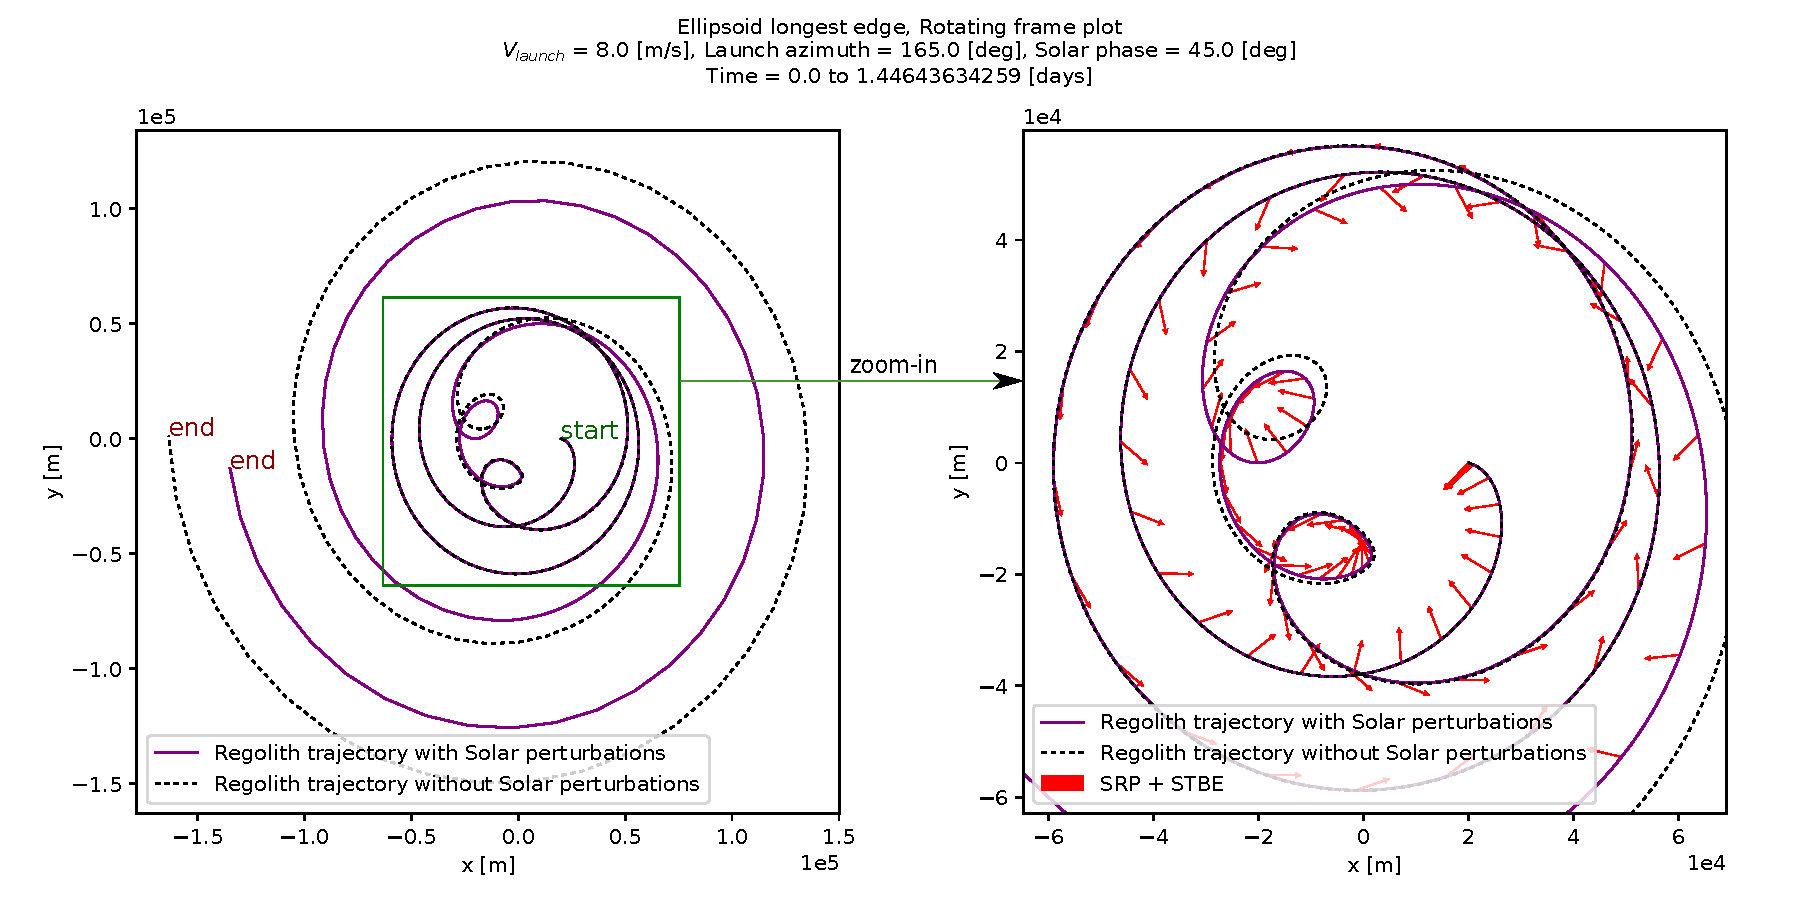
\includegraphics[angle=90, width=\textwidth, height=\textheight, keepaspectratio=true]{longest_edge_perturbations/3.2Density_1cmSize/8ms_165Azimuth_45SolarPhase/comparative_analysis_allPerturbations_rotatingFrame_edited.pdf}
\caption{Rotating frame 2D trajectory (XY plane) of capture regolith for case number 8 in \Cref{tab:LoGSP_1_capture} with direction of the net perturbation vector, compared with the trajectory of a particle launched with the same initial conditions but in absence of Solar perturbations. Particle code LoGSP-1.}
\label{fig:LoGSP_1_capture_case_8_2d_trajectory_comparative_bodyFrame}
\end{figure}
\FloatBarrier
%%%
%%%
\begin{figure}[htb]
\centering
\captionsetup{justification=centering}
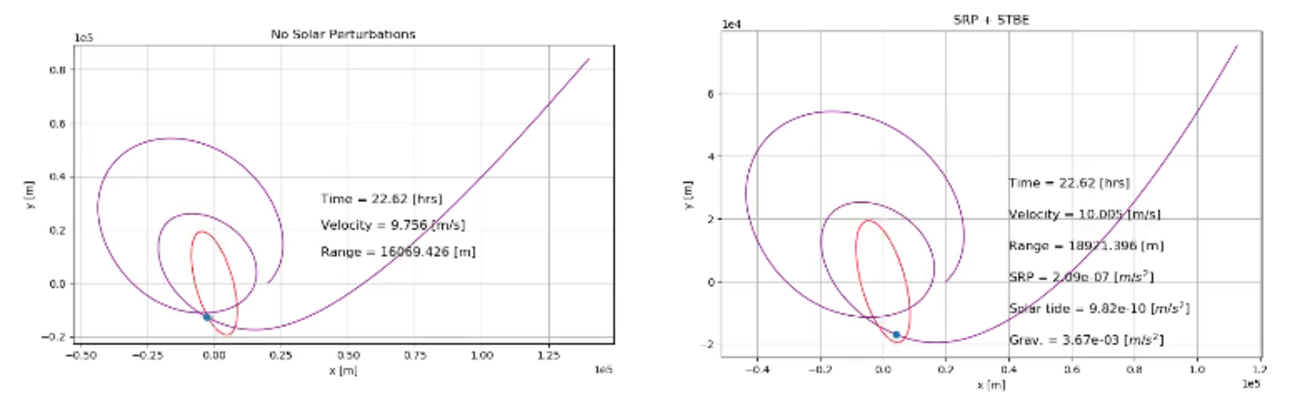
\includegraphics[angle=90, width=\textwidth, height=\textheight, keepaspectratio=true]{longest_edge_perturbations/3.2Density_1cmSize/8ms_165Azimuth_45SolarPhase/comparative_analysis_allPerturbations_phasing_animation_example.pdf}
\caption{Snapshot from animation of the perturbed trajectory of capture case 8 in \Cref{tab:LoGSP_1_capture} compared with that of its unperturbed counterpart. The unperturbed trajectory is still being accelerated at the given instant however the particle in the perturbed trajectory is being decelerated. Particle code LoGSP-1.}
\label{fig:LoGSP_1_capture_case_8_2d_trajectory_comparative_animation_phasing_snapshot}
\end{figure}
\FloatBarrier
%%%
If we look at the trajectory animation in \Cref{fig:LoGSP_1_capture_case_8_2d_trajectory_comparative_animation}, one would notice that at around point \textit{"B"}, the particle in the unperturbed trajectory is being accelerated by the gravitational pull of the asteroid while the particle in the perturbed trajectory is being slowed down. A snapshot of this scenario from the animation is shown in \Cref{fig:LoGSP_1_capture_case_8_2d_trajectory_comparative_animation_phasing_snapshot}. Although this situation does not happen for extended periods of time, but only while approaching point \textit{"B"}, we see that the particle in the unperturbed trajectory has relatively higher velocity while moving forth of point \textit{"B"} and leaving the vicinity of the asteroid, relative to the particle in the perturbed trajectory. The latter thus stays in a capture orbit while the former has enough velocity to escape. A plot for this is shown in \Cref{fig:LoGSP_1_capture_case_8_comparative_inertial_velocity}.

Note that in the capture case just discussed, the magnitude of the perturbing accelerations is much smaller than the gravitational acceleration. The effect of the perturbations on the particle's trajectory is not instantaneous and we can see that in the initial part of the trajectories up until point \textit{"A"} in \Cref{fig:LoGSP_1_capture_case_8_2d_trajectory_comparative_inertialFrame}. Until this point, acceleration due to gravity is in the order of $10^{-4}$, while accelerations due to \gls{SRP} and \gls{STBE} are in the orders of $10^{-7}$ and $10^{-9}$ respectively. Although the perturbing magnitudes are small, but the particles in question are extremely small as well and so over time, the perturbing accelerations add up, leading to a significant change in the trajectory from the unperturbed one.
%%%
\begin{figure}[htb]
\centering
\captionsetup{justification=centering}
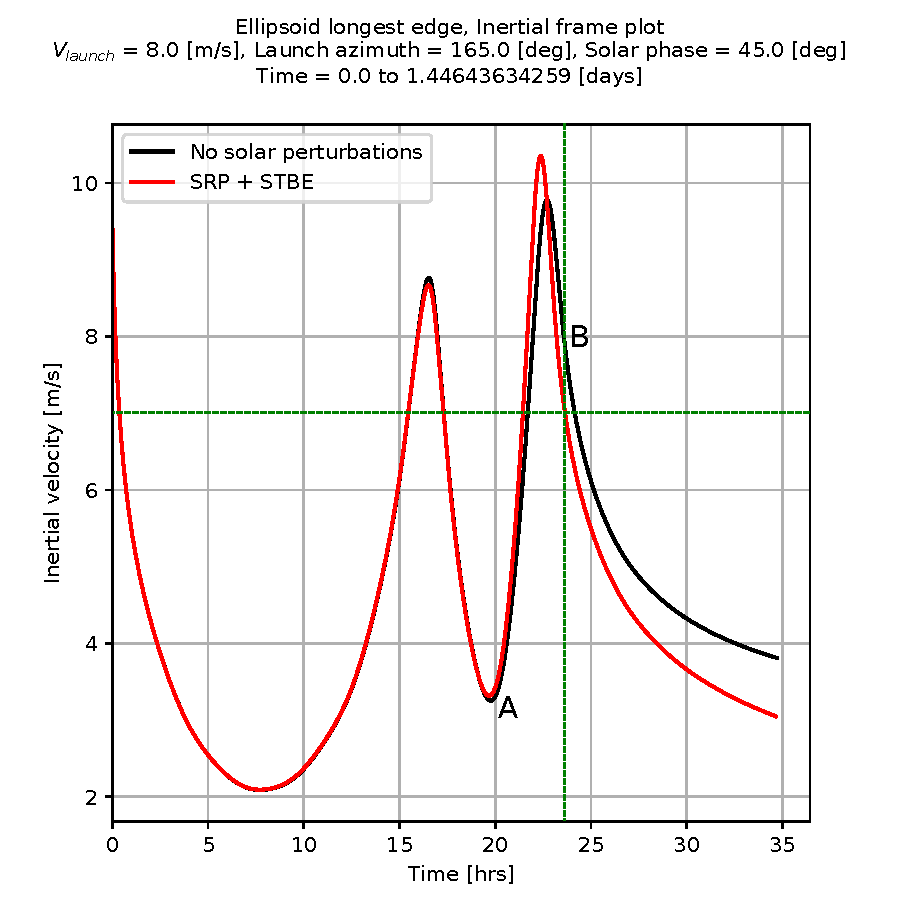
\includegraphics[width=\textwidth, height=0.5\textheight, keepaspectratio=true]{longest_edge_perturbations/3.2Density_1cmSize/8ms_165Azimuth_45SolarPhase/comparative_analysis_allPerturbations_inertialVelocity_edit.pdf}
\caption{Inertial velocity of the perturbed trajectory of capture case 8 in \Cref{tab:LoGSP_1_capture} compared with that of its unperturbed counterpart. The trajectories are shown for the time it takes for the particle in the unperturbed trajectory to escape. Particle code LoGSP-1.}
\label{fig:LoGSP_1_capture_case_8_comparative_inertial_velocity}
\end{figure}
\FloatBarrier
%%%
%%%
\begin{figure}[htb]
\centering
\captionsetup{justification=centering}
\subfloat[]{
    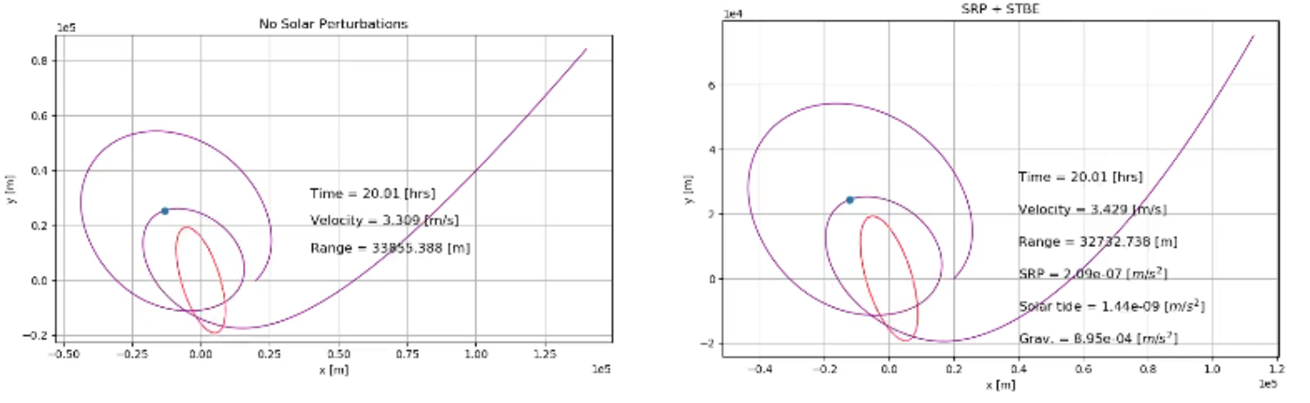
\includegraphics[angle=90, keepaspectratio]{longest_edge_perturbations/3.2Density_1cmSize/8ms_165Azimuth_45SolarPhase/comparative_analysis_animated_trajectory_snippet_initial_differences.pdf}
    \label{fig:LoGSP_1_capture_case_8_2d_comparative_animation_snippet}
}
\vline\vline
\subfloat[]{
    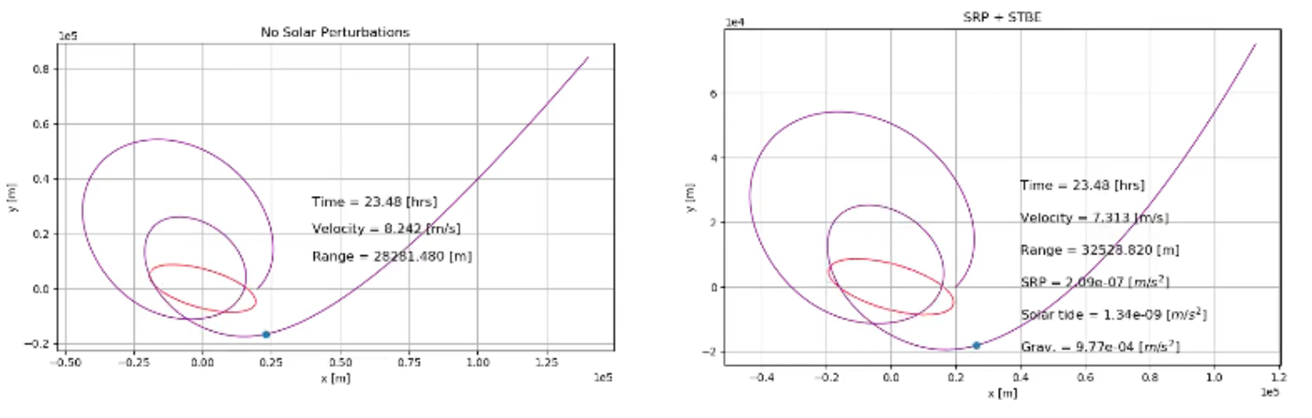
\includegraphics[angle=90, keepaspectratio]{longest_edge_perturbations/3.2Density_1cmSize/8ms_165Azimuth_45SolarPhase/comparative_analysis_animated_trajectory_snippet_escape_point.pdf}
    \label{fig:LoGSP_1_capture_case_8_2d_comparative_animation_phasingExample}
}
\caption{Animation snippets of the inertial frame 2D trajectory (XY plane) of capture regolith for case number 8 in \Cref{tab:LoGSP_1_capture}. The bottom two plots are for the case when Solar perturbations were omitted from the simulation and the top two plots includes them. Note the differences in the range to the particle and its velocity for the same time stamp and rotational state of the asteroid. Particle code LoGSP-1.}
\label{fig:LoGSP_1_capture_case_8_comparative_animation_snapshots}
\end{figure}
\FloatBarrier
%%%
We see a similar effect when we look at capture case number 5 from \Cref{tab:LoGSP_1_capture}. The inertial frame trajectory, both perturbed and unperturbed, for it are shown in \Cref{fig:LoGSP_1_capture_case_5_2d_trajectory_comparative_inertialFrame}. With Solar perturbations removed from the simulation, the initial conditions for this particle result in it getting launched on a highly elliptical orbit and eventually crashing onto the surface of the asteroid after 96 days. The particle, however, avoids this fate when Solar perturbations are included in the simulation. In \Cref{fig:LoGSP_1_capture_case_5_2d_trajectory_comparative_inertialFrame}, it can be clearly seen that the direction of the perturbing acceleration due to \gls{SRP} and \gls{STBE} is consistent with how the trajectory departs from its unperturbed counterpart. The trajectories are shown only for the time it takes for the particle in the unperturbed trajectory to re-impact the surface of the asteroid. We show this case to highlight the effect perturbations have on a trajectory destined for re-impact, unlike the escape scenario discussed previously. We see drastic changes in the perturbed trajectory from the unperturbed one because when the particle is far away from the asteroid, the perturbing acceleration magnitude is of the same order as that of the gravitational acceleration.
% As a thought experiment, we see how the Solar phase angle at the time of launch is important in deciding the final fate of the regolith. We look at \Cref{fig:LoGSP_1_capture_case_5_2d_trajectory_comparative_srpEscape}, where the particle launch conditions are the same as that for the perturbed simulation in \Cref{fig:LoGSP_1_capture_case_5_2d_trajectory_comparative_inertialFrame} except that the initial Solar phase angle is 45.0 [deg] instead of 315.0 [deg]. The former results in an escape situation as the particle is just whisked away by the impeding \gls{SRP}.
%%%
\begin{figure}[htb]
\centering
\captionsetup{justification=centering}
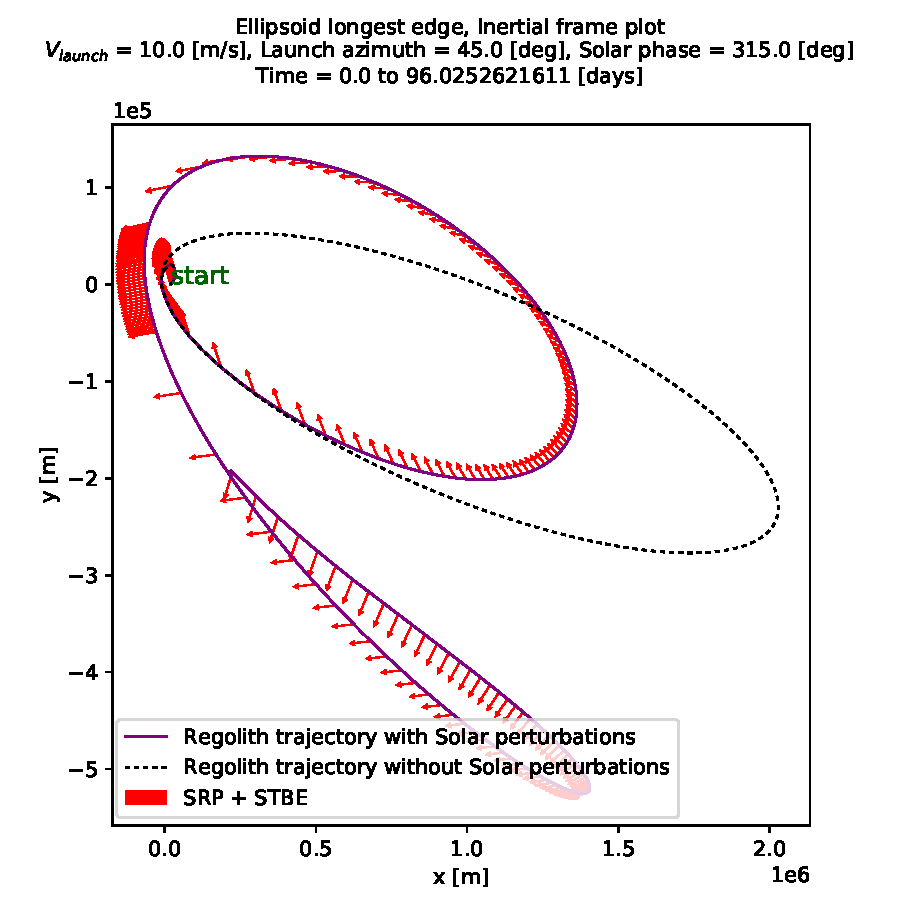
\includegraphics[width=\textwidth, height=0.5\textheight, keepaspectratio=true]{longest_edge_perturbations/3.2Density_1cmSize/singlePlot_comparative_PerturbationVector_10ms_45Azimuth_315SolarPhase_inertialFrame.pdf}
\caption{Inertial frame 2D trajectory (XY plane) of capture regolith for case number 5 in \Cref{tab:LoGSP_1_capture} with direction of \gls{SRP} perturbation vector compared with the trajectory of a particle launched with the same initial conditions but in absence of Solar perturbations. Trajectories shown for as long as it takes the unperturbed trajectory Particle code LoGSP-1.}
\label{fig:LoGSP_1_capture_case_5_2d_trajectory_comparative_inertialFrame}
\end{figure}
\FloatBarrier
%%%
%%%
% \begin{figure}[htb]
% \centering
% \captionsetup{justification=centering}
% % another option for includegraphics - keepaspectratio
% 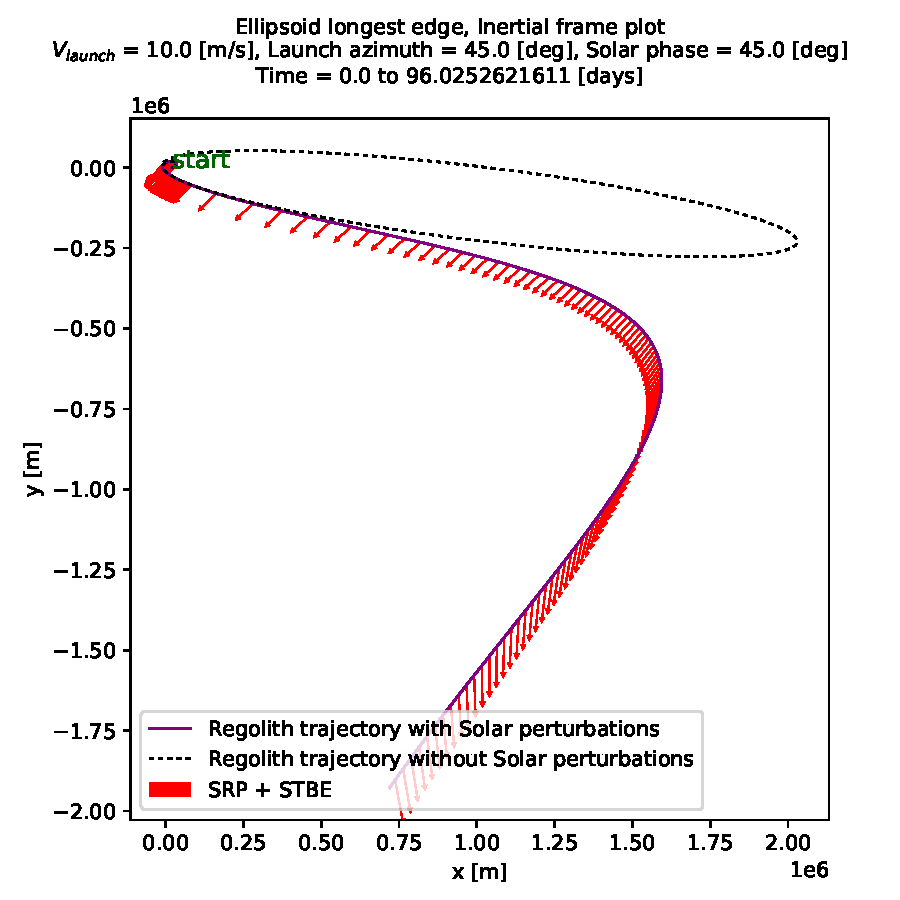
\includegraphics[width=\textwidth, height=0.5\textheight, keepaspectratio=true]{longest_edge_perturbations/3.2Density_1cmSize/srpEscape_comparative_10ms_45Azimuth_45SolarPhase_inertialFrame.pdf}
% \caption{Inertial frame 2D trajectory (XY plane) of capture regolith for same launch velocity and launch azimuth as that of capture case number 5 in \Cref{tab:LoGSP_1_capture} but a different Solar phase angle of 45.0 [deg]. Particle code LoGSP-1.}
% \label{fig:LoGSP_1_capture_case_5_2d_trajectory_comparative_srpEscape}
% \end{figure}
% \FloatBarrier
%%%

\subsubsection{Final fate behavior of different regolith types}
For simulations accounting Solar perturbations, the discussion so far has been about how perturbations affect particle motion and specifically the capture scenario, relative to a particle in an unperturbed simulation. We did this detailed analysis for a single particle type only, namely LoGSP-1 from \Cref{tab:area_to_mass_ratio}. We shall now look into the final fate behavior of all the regolith types mentioned in \Cref{tab:area_to_mass_ratio} to understand how particle motion is affected for different densities and sizes. The simulations were conducted one-by-one for each regolith type, in the same manner as described earlier for particle LoGSP-1. All particles were launched from the longest edge of the asteroid.


